
\documentclass[sigconf]{acmart}

%%
%% \BibTeX command to typeset BibTeX logo in the docs
\AtBeginDocument{%
  \providecommand\BibTeX{{%
    Bib\TeX}}}



%% Rights management information.  This information is sent to you
%% when you complete the rights form.  These commands have SAMPLE
%% values in them; it is your responsibility as an author to replace
%% the commands and values with those provided to you when you
%% complete the rights form.
\setcopyright{none}
\copyrightyear{}
\acmYear{}
\acmDOI{}

\acmConference[Master Thesis]{Department of Statistics, University of Chicago}{April 19th, 2024}{Chicago, IL}
\acmISBN{}

%%
%% Submission ID.
%% Use this when submitting an article to a sponsored event. You'll
%% receive a unique submission ID from the organizers
%% of the event, and this ID should be used as the parameter to this command.
%%\acmSubmissionID{123-A56-BU3}

%%
%% For managing citations, it is recommended to use bibliography
%% files in BibTeX format.
%%
%% You can then either use BibTeX with the ACM-Reference-Format style,
%% or BibLaTeX with the acmnumeric or acmauthoryear sytles, that include
%% support for advanced citation of software artefact from the
%% biblatex-software package, also separately available on CTAN.
%%
%% Look at the sample-*-biblatex.tex files for templates showcasing
%% the biblatex styles.
%%

%%
%% The majority of ACM publications use numbered citations and
%% references.  The command \citestyle{authoryear} switches to the
%% "author year" style.
%%
%% If you are preparing content for an event
%% sponsored by ACM SIGGRAPH, you must use the "author year" style of
%% citations and references.
%% Uncommenting
%% the next command will enable that style.
%%\citestyle{acmauthoryear}

\usepackage{booktabs}
\usepackage{tabulary}
\usepackage{graphicx}
\usepackage{subcaption}
\usepackage{multirow}
\usepackage{longtable}
\usepackage{supertabular}
\usepackage{setspace}
\usepackage{float}
\usepackage[english]{babel}
\usepackage{amsthm}
\usepackage{hyperref}
\usepackage{amsmath}  % Required for math features
\usepackage{amssymb}  % Required for \mathbb and other symbols
\usepackage{array}    % Required for advanced table features
\usepackage{fancyhdr}
\usepackage{makecell} 

\newcommand{\Prob}[1]{\mathbb{P}\left(#1\right)}

\setlength{\floatsep}{5pt}
\setlength{\textfloatsep}{5pt}
\setlength{\intextsep}{5pt}

% Setting up the page style for headers and footers
\pagestyle{fancy}
\renewcommand{\footrulewidth}{0.4pt} % Adds a line above the footer

%%
%% end of the preamble, start of the body of the document source.
\begin{document}


%%
%% The "title" command has an optional parameter,
%% allowing the author to define a "short title" to be used in page headers.
\title{Examining the Interplay Between Politicians' Facial Expressions in Media Images and News Corporation Bias}

%%
%% The "author" command and its associated commands are used to define
%% the authors and their affiliations.
%% Of note is the shared affiliation of the first two authors, and the
%% "authornote" and "authornotemark" commands
%% used to denote shared contribution to the research.


\author{Chenfeng Li}
\email{cfli@uchicago.edu}
\affiliation{%
  \institution{Department of Statistics, University of Chicago}
  \city{Chicago}
  \state{IL}
  \country{USA}
}

%%
%% By default, the full list of authors will be used in the page
%% headers. Often, this list is too long, and will overlap
%% other information printed in the page headers. This command allows
%% the author to define a more concise list
%% of authors' names for this purpose.
\renewcommand{\shortauthors}{Chenfeng Li}

%%
%% The abstract is a short summary of the work to be presented in the
%% article.
\begin{abstract}
   This study explores the interplay between the facial expressions of influential American politicians in media imagery and the political bias of the respective news corporations. We hypothesize that news organizations might preferentially select images that portray politicians with specific emotional expressions to reinforce their editorial biases. Our research involves analyzing approximately one million image URLs from varied news sources to identify and assess the facial expressions of politicians, correlating these expressions with the media's known political orientations. By employing facial recognition and expression analysis, followed by classification and dimensionality reduction techniques, we aim to uncover potential patterns that indicate a bias in visual representation. This research seeks to offer insights into the subtle ways media bias can manifest in the portrayal of political figures, contributing to a deeper understanding of media influence on public perception.
\end{abstract}

%%
%% The code below is generated by the tool at http://dl.acm.org/ccs.cfm.
%% Please copy and paste the code instead of the example below.
%%
% \begin{CCSXML}
% <ccs2012>
%  <concept>
%   <concept_id>00000000.0000000.0000000</concept_id>
%   <concept_desc>Do Not Use This Code, Generate the Correct Terms for Your Paper</concept_desc>
%   <concept_significance>500</concept_significance>
%  </concept>
%  <concept>
%   <concept_id>00000000.00000000.00000000</concept_id>
%   <concept_desc>Do Not Use This Code, Generate the Correct Terms for Your Paper</concept_desc>
%   <concept_significance>300</concept_significance>
%  </concept>
%  <concept>
%   <concept_id>00000000.00000000.00000000</concept_id>
%   <concept_desc>Do Not Use This Code, Generate the Correct Terms for Your Paper</concept_desc>
%   <concept_significance>100</concept_significance>
%  </concept>
%  <concept>
%   <concept_id>00000000.00000000.00000000</concept_id>
%   <concept_desc>Do Not Use This Code, Generate the Correct Terms for Your Paper</concept_desc>
%   <concept_significance>100</concept_significance>
%  </concept>
% </ccs2012>
% \end{CCSXML}

% \ccsdesc[500]{Do Not Use This Code~Generate the Correct Terms for Your Paper}
% \ccsdesc[300]{Do Not Use This Code~Generate the Correct Terms for Your Paper}
% \ccsdesc{Do Not Use This Code~Generate the Correct Terms for Your Paper}
% \ccsdesc[100]{Do Not Use This Code~Generate the Correct Terms for Your Paper}

%%
%% Keywords. The author(s) should pick words that accurately describe
%% the work being presented. Separate the keywords with commas.

%%
%% Keywords. The author(s) should pick words that accurately describe
%% the work being presented. Separate the keywords with commas.
\keywords{News CorporationMedia Bias, Political Communicationians, Facial Recognition, Facial Expression Recognition}
%% A "teaser" image appears between the author and affiliation
%% information and the body of the document, and typically spans the
%% page.



%%
%% This command processes the author and affiliation and title
\maketitle

\section{Introduction}

In the contemporary media landscape of the United States, news corporations commonly exhibit a political bias that skews either progressive (left-leaning) or conservative (right-leaning). On their digital platforms, these outlets frequently utilize photographs of politicians to enhance the visual appeal of their content. This research investigates whether news corporations with distinct political biases select images of influential politicians that depict varying facial expressions. For instance, this study examines whether Donald Trump is portrayed with a more hostile expression in progressive media as opposed to a more composed demeanor in conservative outlets.

We begin with an overview of recent studies on the political bias of news corporations, the impact of image selection on reader perception, and the methodologies for facial expression analysis. In Section~\ref{sec:data}, we introduce the dataset utilized for this research, including details on data acquisition and preprocessing techniques.

In Section~\ref{sec:method}, we outline the methodologies employed to extract and analyze facial expressions from the dataset. This process involves three steps: initially, we retrieve images of politicians from Wikimedia and Wikipedia and use a facial recognition model called FaceNet \cite{facenet} to generate embedding vectors of their faces, subsequently training a name recognition model, which is classification model with their names as labels. Next, for targeted influential politicians, in each image from the dataset, we verify the presence of their faces with the name recognition model and prompts, extracting face crops when applicable. Finally, these face crops are analyzed using an expression recognition model called Residual Masking Network (RMN)\cite{rmn} to obtain emotion logits, which are then stored for analysis.

The results are presented in Section~\ref{sec:results}, where we analyze emotion logits based on the news corporations and the overall political bias. We employ dimension reduction techniques to visualize the emotion logits for various politicians and develop classification models to determine whether the facial expressions in photos can be distinguished by the source of the images.

In Section~\ref{sec:discussion}, we discuss the challenges encountered during the research, the protential reasoning from the experiment results and propose improvements for future studies, and in Section~\ref{sec:conclusion} we summarize the conclusions. Additionally, we provide codes to facilitate the reproduction of this research.

\vspace{-7pt}

\section{Background}\label{sec:background}

The inherent political bias of news corporations is well-documented. This bias can stem from various possible sources, including the political ideologies of journalists and editors, economic interests or funding sources of the corporations, and the editorial choices made to cater to specific reader groups \cite{theorymediabias}. Economists Gentzkow and Shapiro argue that consumer preferences significantly influence media slant \cite{WhatDrivesMediaSlant}. While some level of media bias is inevitable and even acceptable, reflecting broader social structures and cultural values \cite{historyUSNews}, excessive bias can distort public perception and undermine informed decision-making by presenting skewed viewpoints or omitting facts, leading readers away from the truth \cite{theorymediabias}. Analyzing media bias is thus essential for ensuring a well-informed public.

Various researchers and organizations employ diverse methodologies to analyze media bias. For instance, AllSides consistently evaluates major political outlets through editor reviews, blind bias surveys, third-party data, and community feedback \cite{allsidesbias2024}. Ad Fontes Media utilizes a team of 60 trained analysts to rate the political leanings of news sources by scoring individual articles or broadcast episodes, resulting in a media bias chart \cite{adfont}. Quantitative methodologies also abound. Gentzkow and Shapiro, for example, analyzed the U.S. Congress Record to identify phrases more commonly used by Democrats or Republicans, using these findings to calculate a political lean index for news outlets \cite{WhatDrivesMediaSlant}. Moreover, recent studies increasingly leverage language models; Guo, for instance, fine-tuned a masked language model on news articles from politically polarized topics to predict masked tokens and infer the relative biases of these outlets \cite{MLM}.

The role of images in news media is particularly influential. A 2009 study by Grabe and Bucy highlighted the significant impact of image use, often exceeding the influence of text \cite{imagebite}. News corporations might select photos of politicians exhibiting specific behaviors or facial expressions, or manipulate the angle and composition of photographs to shape viewers' perceptions. For example, during an election, a candidate might be portrayed positively in photographs, while their opponent is shown in less flattering contexts, potentially biasing viewers even when the accompanying text is neutral \cite{imagebite}. Rodriguez and Dimitrova introduced the concept of visual framing in 2011, which examines how visuals in news images are selected, composed, and presented to convey specific interpretations of news stories or events, thereby structuring the interpretation and emotional response of the audience \cite{visualframing}.

In this research, we specifically focuses on the variety of facial expressions of politicians across different news corporations. In 1992, psychologist Paul Ekman proposed that there are six basic and universally distinguishable facial emotions: anger, disgust, happiness, sadness, fear, and surprise \cite{emotions}. Building on Ekman’s work, Du et al. argued for the existence of fifteen distinct compound facial emotions created by combining the muscle movements of the six basic emotions, such as happily surprised or fearfully surprised, thereby enabling a quantitative classification of emotions \cite{compoundemotion}.




\section{Data Preparation}\label{sec:data}
\subsection{Data Cleaning}\label{sec:clean}
The dataset used in this research was provided by Prof. James Turk from the Department of Computer Science at the University of Chicago and the latest update was on September 7, 2023 \cite{dataset}. It comprises 1,019,845 image samples extracted from various news articles. Each sample includes an image URL and may also contain associated texts such as the article title, image caption, and alternative text (displayed when the original image cannot be shown properly on the website). The structure of the dataset is detailed in Table ~\ref{tab:metadata}.

\setlength{\textfloatsep}{0pt}
\begin{table}[t]
  \begin{center}
  \renewcommand{\arraystretch}{1.5}
  \begin{tabular}{|l|p{5.5cm}|}
    \hline
    \textbf{Column} & \textbf{Example} \\
    \hline
    UUID & b85aa64d-411f-11ee-a96e-33dec8f414a2 \\
    \hline
    Title of Article & Laura Loomer Files RICO Case Against Twitter and Facebook \\
    \hline
    Image URL & https://media.breitbart.com/media/2020/07/ \newline Jack-Dorsey-and-Twitter-employees.jpg \\
    \hline
    Image Caption & Jack Dorsey and Twitter employees (@Jack/Twitter) \\
    \hline
    Alternative Text & Jack Dorsey and Twitter employees \\
    \hline
    Image Type & ImageType.main \\
    \hline
  \end{tabular}
  \caption{Metadata of the dataset. \newline The Column Title of Article, Image Caption, and Alt Text of Image may be empty.}
  \label{tab:metadata}
  \end{center}
\end{table}


In this dataset, samples lacking a URL, those with invalid URLs (not starting with "http:" or "https:"), and duplicates were removed. The definition of duplicates in this context is nuanced. In this dataset, as each UUID can correspond to multiple images, it is not a reliable indicator of duplicates \footnote{e.g. 8 different images share the same UUID 3d19261c-406a-11ee-a96e-33dec8f414a2}. Furthermore, the textual elements (title, caption, alternative text) may be absent, which cannot be used as indicators on their own. Intuitively, we considered image URLs as duplicate indicators; however, this approach proved problematic, as media outlets often reuse images from their online galleries across different reports \footnote{e.g. The image URL \href{https://media.cnn.com/api/v1/images/stellar/prod/190801141718-01-donald-trump-july-30-2019.jpg?q=x_0,y_45,h_1259,w_2238,c_crop/w_850}{\underline{https://media.cnn.com/api/v1/images/stellar/prod/190801141718}\newline \underline{-01-donald-trump-july-30-2019.jpg?q=x\_0,y\_45,h\_1259,w\_2238,c\_crop/w\_850}} \newline appears twice in unique samples}. Thus, a sample is considered a duplicate only if it shares the same image URL and the title, image link, caption, and alternative texts with another.



Another challenging aspect of duplication removal involves images from the same article that appear under different URLs \footnote{e.g. The two images sharing the UUID 000590e6-3d60-11ee-a96e-33dec8f414a2 come from the same article, where the first one is resized from the second one}. These instances typically arise due to responsive web design or optimizations for the web searching. We address these cases separately, as they do not impact the research findings, which we discuss further in Section ~\ref{sec:duplicates}.

\subsection{Source Analysis}
Following data cleaning, we identified the source of each image based on the second-level domain of the URL (the section before the top-level domain, such as ".com", ".org", or ".net"). For example, the image URL \underline{https://static.\textbf{politico}.com/capny/sites/default/files/a-} \underline{Uber\%20HQ\_0.png} is associated with the Politico, whereas \underline{https://} \underline{\textbf{dailycaller}.com/wp-content/uploads/2018/07/Michael-Ian-Black} \newline \underline{-Twitter-4.jpg} originates from The Daily Caller.. 

After determining the sources and filtering out images not from news corporations (e.g., those from social media or online galleries), and integrating media bias ratings from AllSides \cite{allsides2024}, the refined dataset contained 842,232 samples. The distribution of these samples across various news corporations, categorized by their political bias, is summarized in Table ~\ref{tab:source}.

\begin{table}[ht]
  \centering
  \renewcommand{\arraystretch}{1.2}
  \label{tab:politics_bias}
  \begin{tabular}{|l|l|r|}
    \hline
    \textbf{Corporation} & \textbf{Politics Bias} & \textbf{Sample Size} \\ \hline
    CNN & Left & 21,401 \\ \hline
    NPR & Left & 76,385 \\ \hline
    Politico & Left & 312,448 \\ \hline
    APNews & Left & 4,658 \\ \hline
    Washington Times & Right & 104,421 \\ \hline
    DailyCaller & Right & 145,019 \\ \hline
    FoxNews & Right & 96,702 \\ \hline
    Breitbart & Right & 81,152 \\ \hline
    Others & N/A & 43 \\ \hline
  \end{tabular}
  \caption{Source of samples}
  \label{tab:source}
\end{table}


\section{Methodologies}\label{sec:method}

\begin{figure}
    \centering
    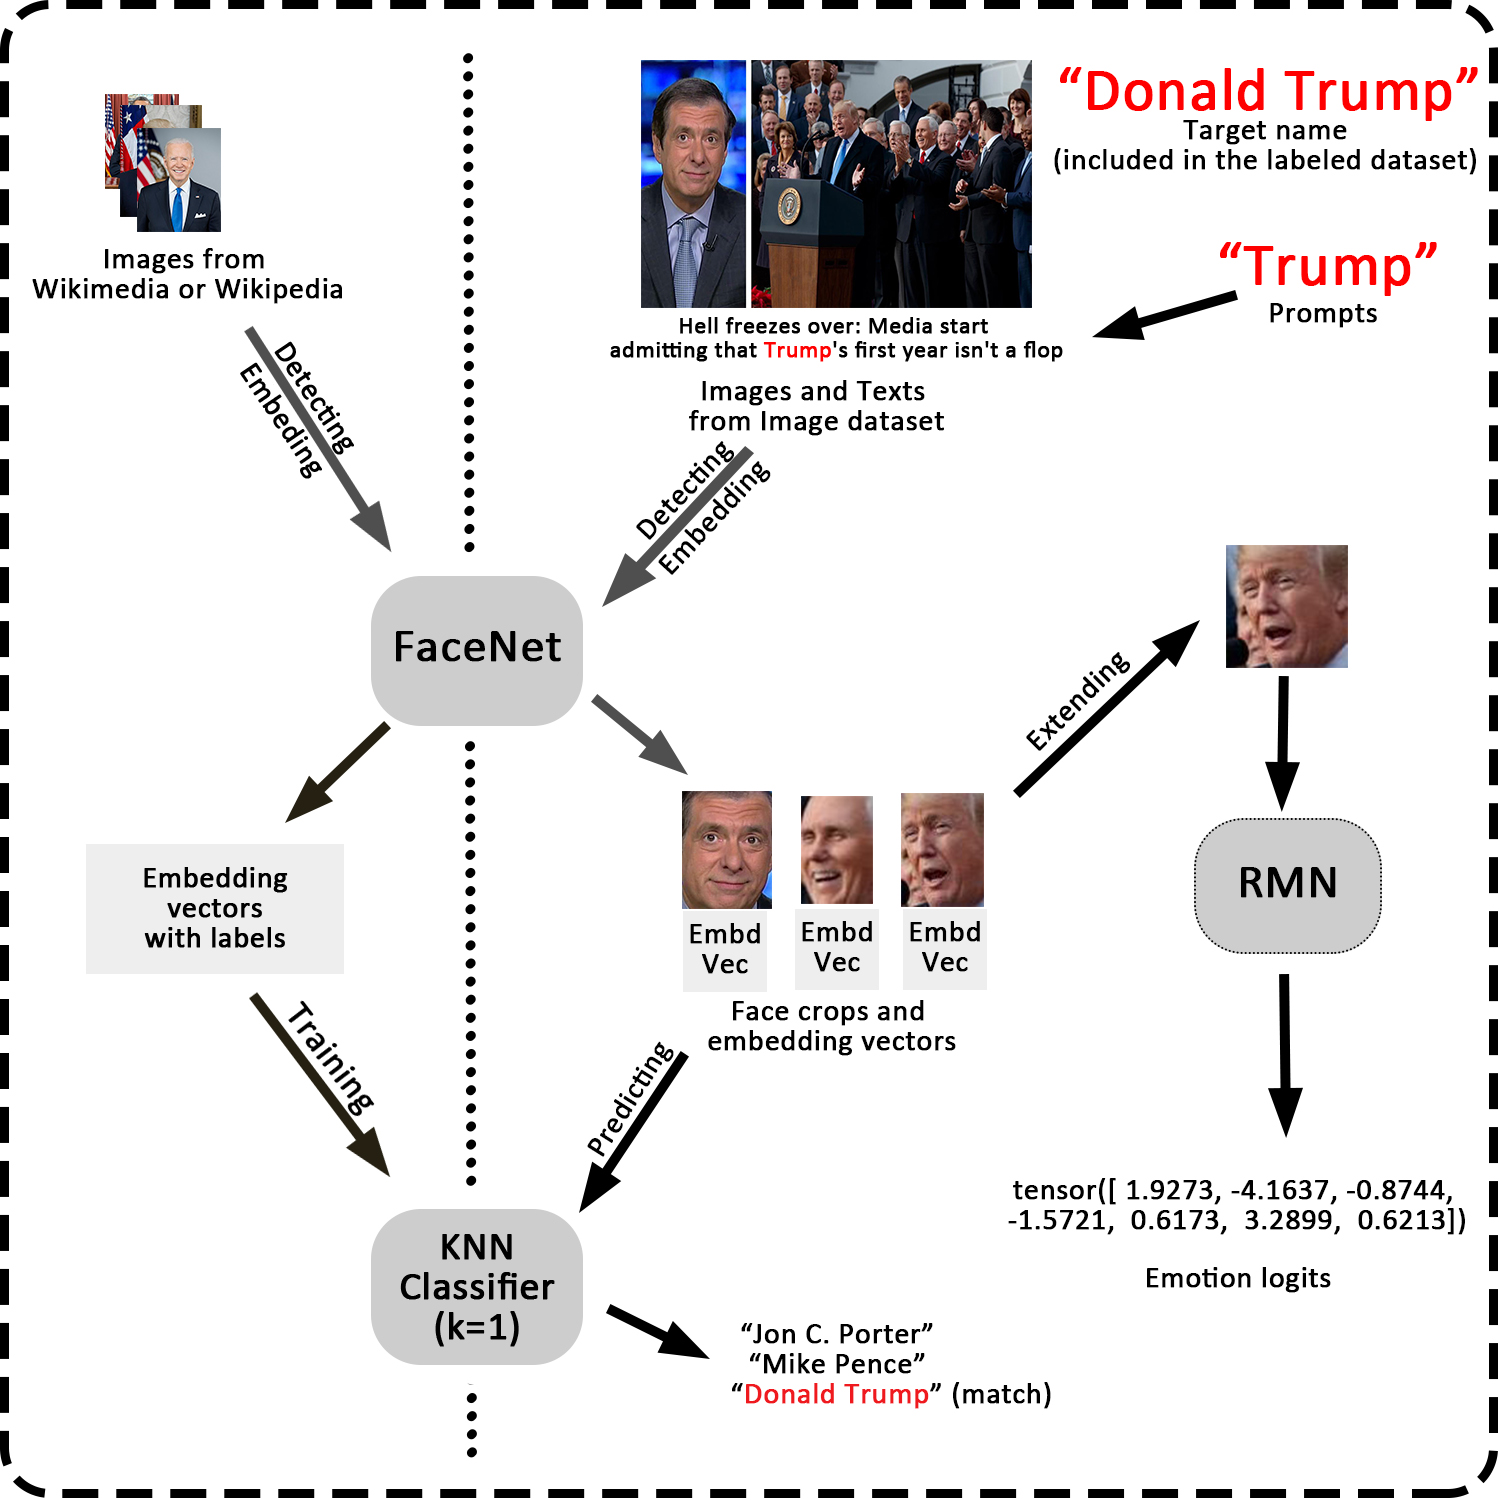
\includegraphics[width=.5\textwidth]{assets/thesis.jpg}
    \caption{Overview of converting images from the dataset to emotion logits with name of politicians}
    \label{fig:overview}
    \vspace{10pt}
\end{figure}

\subsection{Name Recognition Model}

At the outset of this experimental section, we introduce the FaceNet model, a robust facial recognition system developed by researchers affiliated with Google \cite{facenet}. For our research, we employed the PyTorch implementation of the FaceNet model by Tim Esler et al. \cite{facenetpytorch}. This model comprises two components: the facial detection segment uses the Multi-task Cascaded Convolutional Networks (MTCNN), proposed by Zhang et al. in 2016, which is a three-stage Convolutional Neural Network (CNN) known for its precision in facial detection \cite{mtcnn}. The recognition component utilizes the InceptionResnetV1 model, a CNN that integrates elements from both the Inception architecture and the Residual Network (Resnet), with the Inception architecture playing a pivotal role in FaceNet. Given an image, the output from the MTCNN is a list of facial characteristic matrices and their rectangular coordinates, identifying detected faces. Each matrix is then processed by the InceptionResnetV1 model to produce a face embedding vector of dimension 8631, allowing us to compare the similarity of faces using the Euclidean distance between embedding vectors.


The primary objective of our research is to analyze the emotions of specific politicians from various news corporations. Initially, the content of each image in our dataset was unknown, ranging from news corporation logos and landscapes to photographs of one or multiple people, not all of whom were necessarily politicians. Our initial approach was to identify targeted politicians by searching for their names in the texts associated with each image. However, this method proved inadequate. For instance, not all images with "Hillary Clinton" in the texts actually contained a photo of Mrs. Clinton, and might include other individuals. Moreover, Mrs. Clinton is frequently referred to by various names or titles, such as "Hillary Rodham Clinton," "Mrs. Clinton," "Secretary Clinton," etc. Directly searching for "Hillary Clinton" could result in missing relevant images, while searching for "Clinton" could pull in irrelevant images of other individuals with the same last name.

Before analyzing the dataset described in Section ~\ref{sec:data}, our initial task is to construct a name recognition model. This model first determines if there are faces within an input image and then identifies the names associated with those faces. To achieve this, we require an additional labeled photo dataset that includes both photographs of politicians and their corresponding names. An ideal source for this data is Wikimedia, a sister project to Wikipedia that allows users to create pages of persons and upload relevant images \cite{wikimedia}. Many celebrities with Wikipedia pages also have Wikimedia pages containing relevant images. Additionally, the categorical structure of Wikimedia is particularly useful, as it facilitates easy access to images of individuals within similar groups. Moreover, since Wikimedia pages for some politicians may contain subcategories, which in turn may include further subcategories, we recursively fetched image URLs across all levels up to a depth of three. We systematically fetched image URLs of politicians from the following three categories.

\begin{itemize}
  \item \href{https://commons.wikimedia.org/wiki/Category:21st-century_male_politicians_of_the_United_States}{\underline{Category:21st-century male politicians of the United States}}
  \item \href{https://commons.wikimedia.org/wiki/Category:21st-century_female_politicians_of_the_United_States}{\underline{Category:21st-century female politicians of the United States}}
  \item \href{https://commons.wikimedia.org/w/index.php?title=Category:21st-century_businesspeople_from_the_United_States&oldid=527515279}{\underline{Category:21st-century businesspeople from the United States}}
\end{itemize}

The imageURL-name dataset sourced from Wikimedia now includes image URLs of approximately 2700 politicians. Additionally, there are politicians who are represented on Wikipedia with portrait images on their pages but do not have corresponding Wikimedia pages. To enrich the imageURL-name dataset, we further extracted portrait URLs from Wikipedia, specifically targeting politicians listed under the following two categories:

\begin{itemize}
  \item \href{https://en.wikipedia.org/w/index.php?title=Category:21st-century_American_politicians&oldid=1015022478}{\underline{Category:21st-century American politicians}}
  \item \href{https://en.wikipedia.org/w/index.php?title=Category:21st-century_American_businesspeople&oldid=1110690935}{\underline{Category:21st-century American businesspeople}}

\end{itemize}

To ensure comprehensive coverage, we cross-referenced politicians listed in two Wikipedia categories with those in the previous three Wikimedia categories. For each politician on Wikipedia, we first checked for a Wikimedia page and retrieved image URLs if available. If no Wikimedia page existed, we instead captured the portrait URL from the Wikipedia page and added it to our imageURL-name dataset. Through this process, we examined the pages of 20,707 politicians, ultimately compiling a dataset containing 312,587 URLs from 10,094 politicians, noting that some pages did not contain any image URLs.

Upon gathering the image URLs with names from both Wikimedia and Wikipedia, we needed to verify that the images actually contained the politician's face. Wikimedia galleries conveniently ensure that the first image on a person’s page is a portrait containing exactly one face. We utilized this portrait as the 'control face' for each page, inputting it into the FaceNet model to obtain an embedding vector. We established a similarity threshold of 200. For each embedding vector derived from page images, if the Euclidean distance to the control vector was below this threshold, we identified the face as belonging to the page owner and stored the vector with the owner's name. This threshold was found to be reasonable through extensive testing. To optimize both time and storage, we saved only ten face embedding vectors per politician, including the control vector. This process yielded a face-name dataset with 37,934 face embedding vectors from 9,308 politicians.


With the labeled face-name dataset prepared, we developed a name recognition model using a K-Nearest Neighbors (KNN) algorithm set to \(K=1\). This model predicts the name associated with a new face embedding vector as that of the nearest vector in our dataset. We selected \(K=1\) since some politicians are represented by only one vector (i.e. the control vector). The validation accuracy of this model reached 80.60\%, significantly exceeding the baseline random guessing rate of 0.01\%. There is a concerning that this model is limited to predicting names only within the face-name dataset. In other words, the faces of persons outside the face-name dataset will be always misidentified. We will discuss strategies to address this limitation in the next section.



\subsection{Face Crops for Influential Politicians} \label{sec:facecrops}
In this section, we describe the method for obtaining face crops of influential politicians from different news corporations, utilizing the dataset detailed in Section ~\ref{sec:data}. 

Using Donald Trump as a case study (illustrated in Figure ~\ref{fig:overview}), we begin by specifying the targeted name for which we seek to find face crops, in this case, "Donald Trump". Then we select some prompts closely relevant to Mr. Trump, such as the part of the name or the position. Here we use "Trump" as the single prompt. These prompts are then used to filter the dataset, retaining only those samples whose associated texts contain the selected prompts.

Each image from the filtered dataset is processed through the FaceNet model to extract a list of face crops and their corresponding embedding vectors. These vectors are then fed into the name recognition model. If the model predicts the name of the face as "Donald Trump" and it matches our target name exactly, we store the face embedding vector and face crop coordinate, along with the name and the source news corporation for further emotion analysis. To optimize resource use and reduce processing time, for each politician, we randomly select at most 2,000 face crops from each corporation, as listed in Table ~\ref{tab:source}.

In the subsequent section, we will address three key questions by statistically analyzing the prediction accuracy of the name recognition model:

\begin{enumerate}
\item How can we address the limitations of the name recognition model mentioned in the previous section?
\item Why do we specifically analyze influential politicians, or in other words, politicians who frequently appear in news articles?
\item What is the purpose of using prompts in our methodology?
\end{enumerate}

First, let's consider the scenario where no prompts are used.

For a given face image, let \( n \) represent a name, \( F \) the actual name of the person in the image, \( P \) the name predicted by the name recognition model, and \( D_n \) the event that the name \( n \) is included in the name recognition model. We are particularly interested in \( \Prob{F = n | P = n} \), which is the conditional probability that the actual name of the person is \( n \) given that the model predicts \( n \).

According to Bayesian Theorem:

\begin{align*}
&\Prob{F = n | P = n} \\
&= \Prob{F = n | P = n, D_n} \\
&= \frac{\Prob{P = n | F = n, D_n} \cdot \Prob{F = n|D_n}}{\Prob{P = n | F = n, D_n} \cdot \Prob{F = n|D_n} + \Prob{P = n | F \neq n, D_n} \cdot \Prob{F \neq n|D_n}}
\end{align*}

where
\begin{itemize}
\item \( \Prob{P = n | F = n, D_n}\) is the prediction accuracy of the name recognition model, previously estimated at 0.806.
\item \( \Prob{P = n | F \neq n, D_n} \) is the probability that the name \( n \) is predicted even though the actual name is not \( n \), which we estimate as \( \frac{1}{9308} \) representing the likelihood of a random choice. We use this probability to represent the limitation of name recognition model as in Question (1).
\item \( \Prob{F = n|D_n} \) reflects the frequency of the name 
 \( n \) appearing in the dataset, indicating the exposure level of the politician in news articles.
\end{itemize}

Here are some pairs/‘ between the frequency and the targeted probability:

\begin{table}[H]  % Forces the table to not float, but stay here
\centering  % Centers the table
\begin{tabular}{|c|c|}
\hline
\( \Prob{F=n | D_n} \) & \( \Prob{F=n | P=n} \) \\
\hline
0.01 & 0.987 \\
0.001 & 0.882 \\
0.0001 & 0.429 \\
\hline
\end{tabular}
\caption{Relationship between the frequency of politician appeared on news article and the probability of actual name matched given predicted}
\label{tab:prob_estimates}
\end{table}
\vspace{-20pt}

This table highlights the implications of the second question. For instance, if a politician's name appears in the news with a frequency of 1\%, then when the name is predicted, there is a 98.7\% probability that it is correct. However, if the frequency drops to 0.01\%, the probability of a correct prediction plummets to 42.9\%, indicating a high risk of error. This finding underpins our focus on influential politicians who frequently appear in news articles, as their higher visibility reduces the likelihood of mistaken predictions and ensures a sufficient sample size for robust analysis. Moreover, less influential politicians typically do not provide enough data for a reliable analysis of photo selection biases.

Next, we discuss the advantages of using prompts (Question 3) by examining the benefits they provide in enhancing the accuracy of our model predictions.

Let \( T_n \) represent the set of prompts associated with the individual \( n \). In this analysis, we are specifically interested in \( P(F = n \mid P = n, T_n) \), the conditional probability that the person's actual name is \( n \) given that the name \( n \) is predicted when prompts \( T_n \) are used.

It is important to note that, conditional on the true name \( F \), the prediction \( P \) and the prompts \( T_n \) are statistically independent. Therefore, we can express the probability as:

\begin{align*}
&\Prob{F = n \mid P = n, T_n}\\
&= \Prob{F = n \mid P = n, T_n, D_n} \\
&= \frac{A*B }{A*B + C*D}
\end{align*}

where 
\begin{itemize}
    \item \( A = \Prob{P = n \mid F = n, T_n, D_n} = \Prob{P = n \mid F = n, D_n} \) represents the prediction accuracy of the name recognition model.
    \item \( B = \Prob{F = n \mid T_n, D_n} \) is the frequency of \( n \) appearing in images associated with the prompts.
    \item \( C = \Prob{P = n \mid F \neq n, T_n, D_n} = \Prob{P = n \mid F \neq n, D_n} \) is the probability of incorrectly predicting \( n \) given the actual name is not \( n \).
    \item \( D = \Prob{F \neq n \mid T_n, D_n} = 1-B \)
\end{itemize}

Note that the term \(A\) and \(C\) also appear in the equations where the prompts are not used. The significant factors between without and with the usage of prompts are \(\Prob{F = n \mid T_n, D_n}\) and \(\Prob{F = n \mid T_n, D_n}\). For instance, in the case of Mr. Trump:

\begin{itemize}
    \item \(\Prob{F = n \mid D_n}\) is the general frequency of Mr. Trump’s face in news articles.
    \item \(\Prob{F = n \mid T_n, D_n}\) is the frequency of Mr. Trump’s face in news articles specifically where the prompt "Trump" appears, such as in article text, captions, or alternative text.
\end{itemize}

Despite the increased probability afforded by using prompts, it is crucial to maintain a focus on influential politicians. This is because, with the narrowed scope induced by prompts, the sample size for less famous politicians decreases significantly. Moreover, the frequency \( \Prob{F = n \mid D_n} \) cannot be too low to maintain a meaningful probability of correct identification:

\[
\Prob{F = n \mid T_n, D_n} \propto \Prob{T_n \mid F = n, D_n} \cdot \Prob{F = n \mid D_n}
\]

This mathematical relationship underscores the need to ensure a reasonable baseline frequency of the politician's appearance in the dataset to effectively utilize prompts for enhancing prediction accuracy.

We applied our process to famous politicians including Joe Biden, Donald Trump, Hillary Clinton, and Barack Obama, covering a range of parties, genders, and races. This resulted in a new dataset comprising the names of the politicians, source news corporations, face embedding vectors, and the rectangular coordinates of each face crop from the original image. We then assessed the quality of the face embedding vectors from each news corporation to determine if they could effectively distinguish between politicians.

For this evaluation, we employed dimensionality reduction techniques—Uniform Manifold Approximation and Projection (UMAP) and Principal Component Analysis(PCA)—to reduce the dimensionality of the embedding vectors from 8631 to 2. This allowed us to visualize the data, labeling each point with the corresponding politician's name. The resulting plots for Politico and the Daily Caller, shown in Figure ~\ref{fig:embd}, illustrate that embedding vectors of the same politician cluster closely together, while vectors representing different politicians are distinctly separated. This confirms that the embedding vectors can clearly distinguish between different politicians.

\begin{figure}
    \centering
    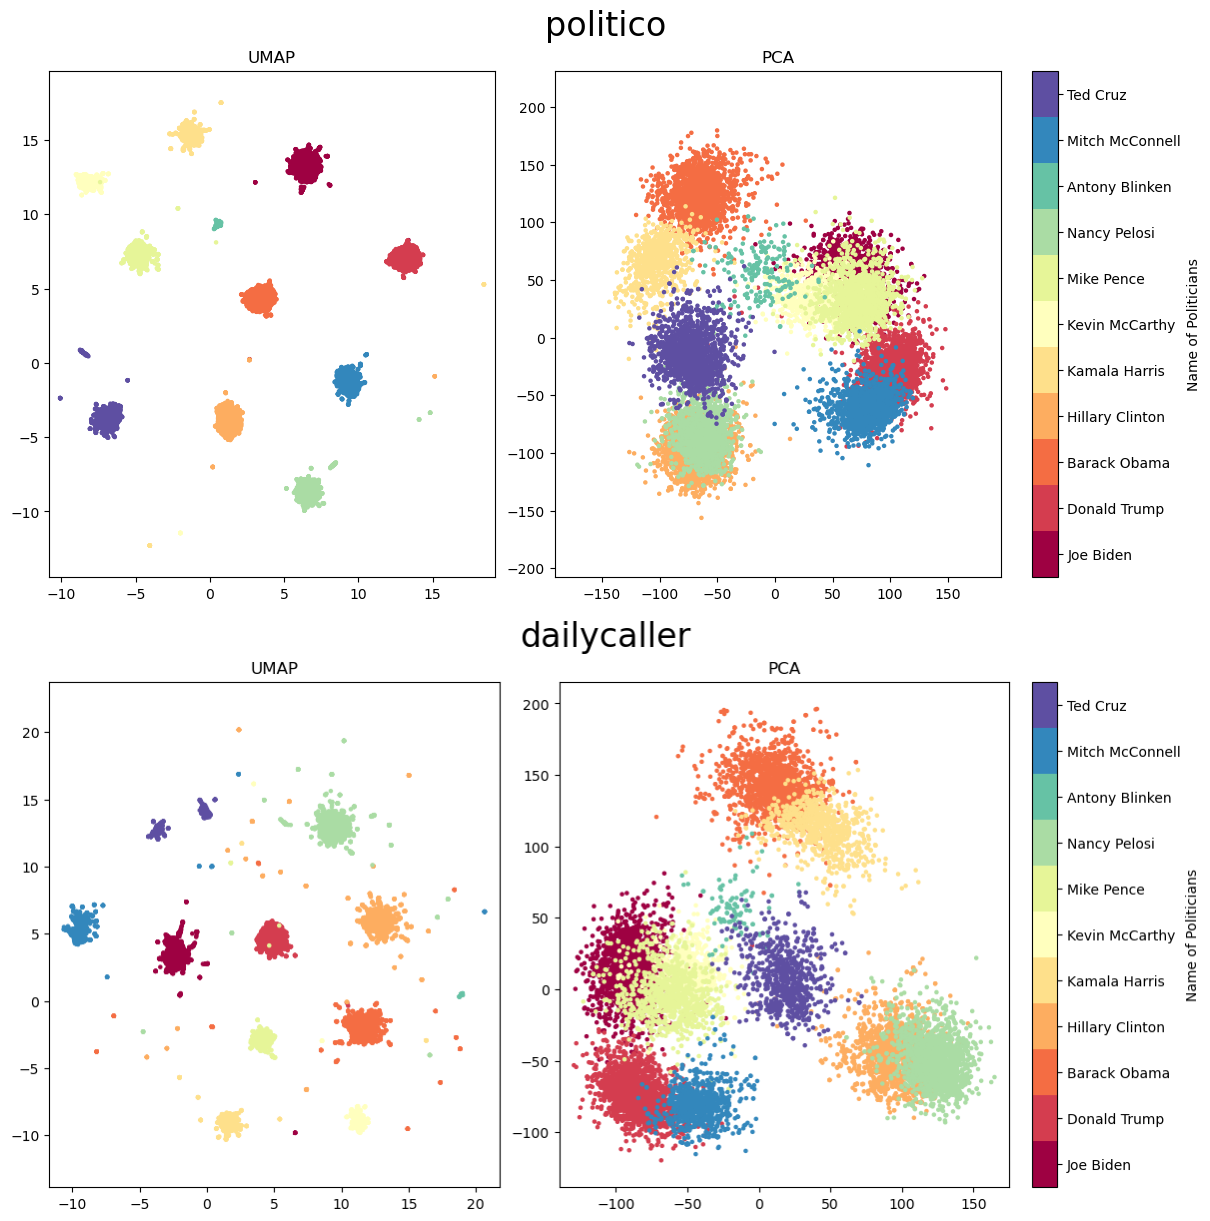
\includegraphics[width=.5\textwidth]{assets/embd.png}
    \caption{Visualization of Face Embedding Vectors}
    \label{fig:embd}
    \vspace{10pt}
\end{figure}



\subsection{Emotion Logits}

After obtaining face crops of specific politicians using the previously described method, the next step involves analyzing their emotions. We recognize that facial expressions can be decomposed into six basic emotions plus a neutral expression \cite{compoundemotion}. Consequently, we represent facial expressions using a seven-dimensional vector, where each entry corresponds to one of these emotional states. This vector is referred to as the emotion logit, and we derive the probability or weight of each emotion by applying the softmax function.

In this study, we employ the Residual Masking Network (RMN), a facial expression recognition (FER) model introduced by Pham et al \cite{rmn}. The core of the RMN consists of four Residual Masking Blocks, each composed of a Residual Layer and a Masking Block. These blocks are part of an innovatively designed CNN architecture. Each input feature map processed by a Residual Masking Block is first refined by the Residual Layer to produce a coarse feature map, and then further refined by the Masking Block to enhance the expression features of the face image. The output of the RMN model for any given image is a seven-dimensional vector of emotion logits, which represent the combination of facial expressions analyzed for each politician.

The RMN model was trained using the Fer2013 dataset, introduced at the 2013 Challenges in Representation Learning by the International Conference on Machine Learning \cite{fer2013}. This dataset comprises 35,887 grayscale images of faces, each 48x48 pixels, labeled with one of the seven emotion categories. Human accuracy for recognizing expressions from this dataset is approximately 65\%. In contrast, the RMN model achieved a validation accuracy of 76.14\% when trained on the Fer2013 dataset, surpassing human performance and marking the highest accuracy reported to our knowledge. This demonstrates the robustness of the RMN model in recognizing facial expressions.

Now, we need to compute the emotion logits from the face crops using the RMN model. Initially, since the coordinates of the face crops are rectangular and the RMN model requires square inputs, we adjust the coordinates by expanding the shorter edges of the rectangle to form a square. The color scale of the face crops is then converted from RGB to grayscale. These pre-processed, gray-scaled, square face crops are subsequently fed into the RMN model to obtain the emotion logits.

% Possible improvement: Example of face crop and expression

After this processing, we have compiled a dataset containing emotion logits derived from their facial expressions, and the corresponding the names of politicians and their associated news corporations. Similar to how we visualized the face embedding vectors in the previous section, we use UMAP and PCA to visualize the emotion logits for the face images came from Politico and The Daily Caller, as shown in Figure ~\ref{fig:emo_logits}. Note that in both visualization methods, the plots resemble clouds where the emotion logits of different politicians may overlap significantly. This overlap is expected as different politicians can exhibit similar expressions. However, it is noticeable that the emotion logits for each politician tend to cluster together, suggesting that each politician has a distinct set of facial expressions they commonly use. This indicates that it is feasible to use emotion analysis to predict the identity of the politicians with non-trivial accuracy.

\begin{figure}
    \centering
    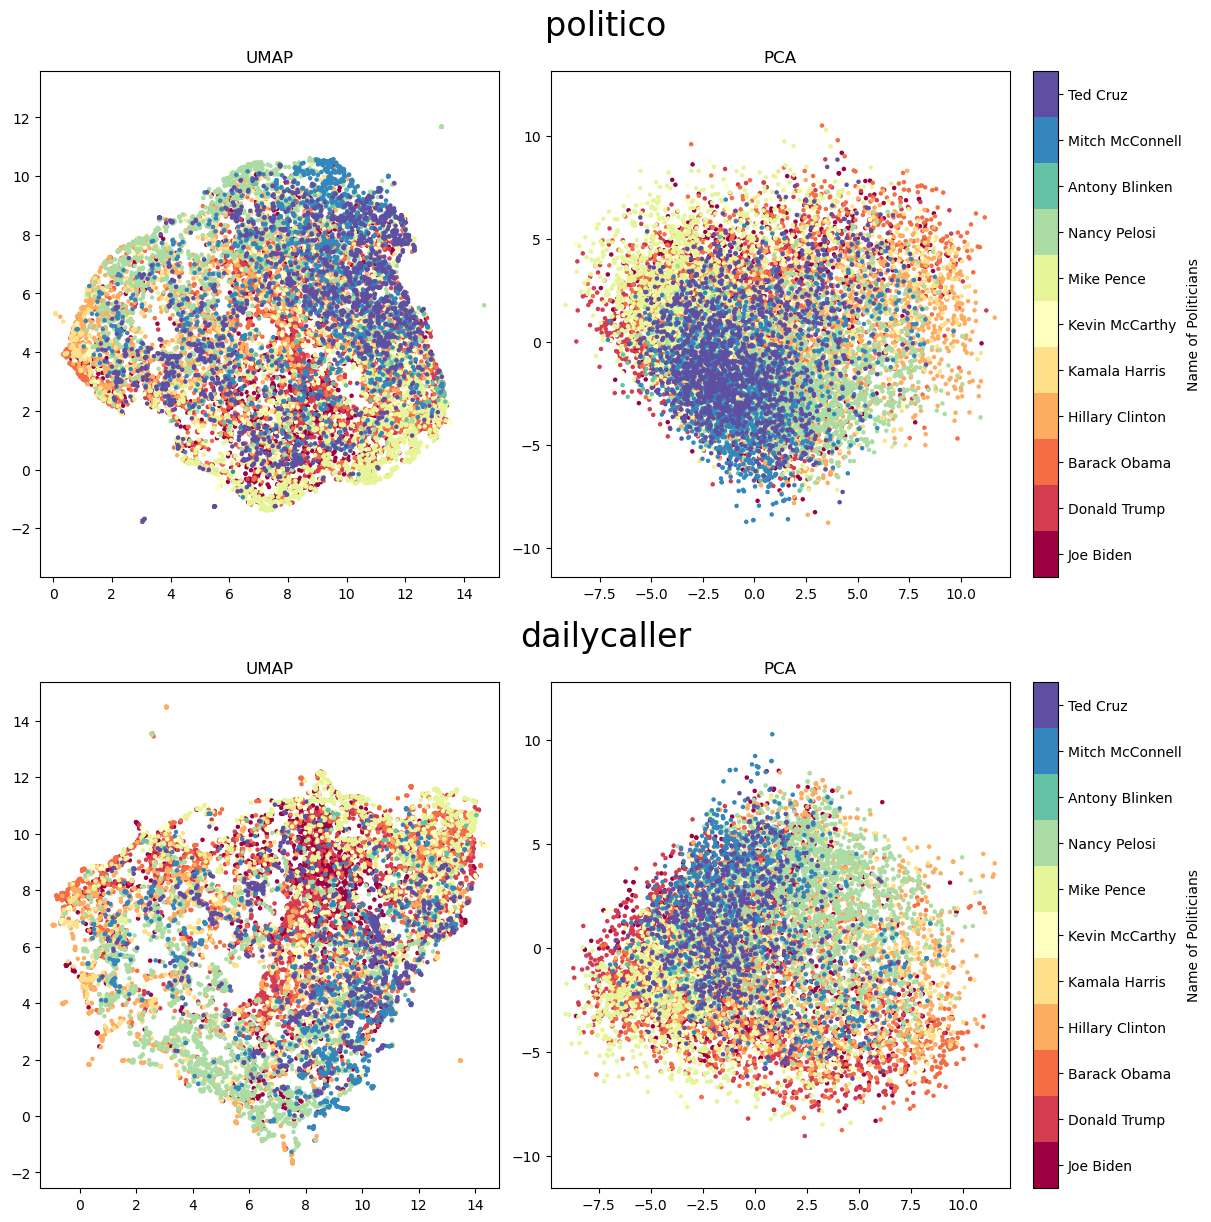
\includegraphics[width=.5\textwidth]{assets/emotion_logit.png}
    \caption{Visualization of Emotion Logits}
    \label{fig:emo_logits}
    \vspace{10pt}
\end{figure}



\section{Results}\label{sec:results}

In this section, we explore the relationship between emotion logits and the source news corporations or their political biases for specific politicians. This analysis involves visualizations and the use of classification models to interpret how facial expressions expressed in images of politicians correlate with the political bias of news corporations. We use emotion logits derived from Joe Biden, Donald Trump, Hillary Clinton, and Barack Obama as our primary examples.

\subsection{Visualization of Emotion Logits}\label{sec:vis}

\begin{figure}
    \centering
    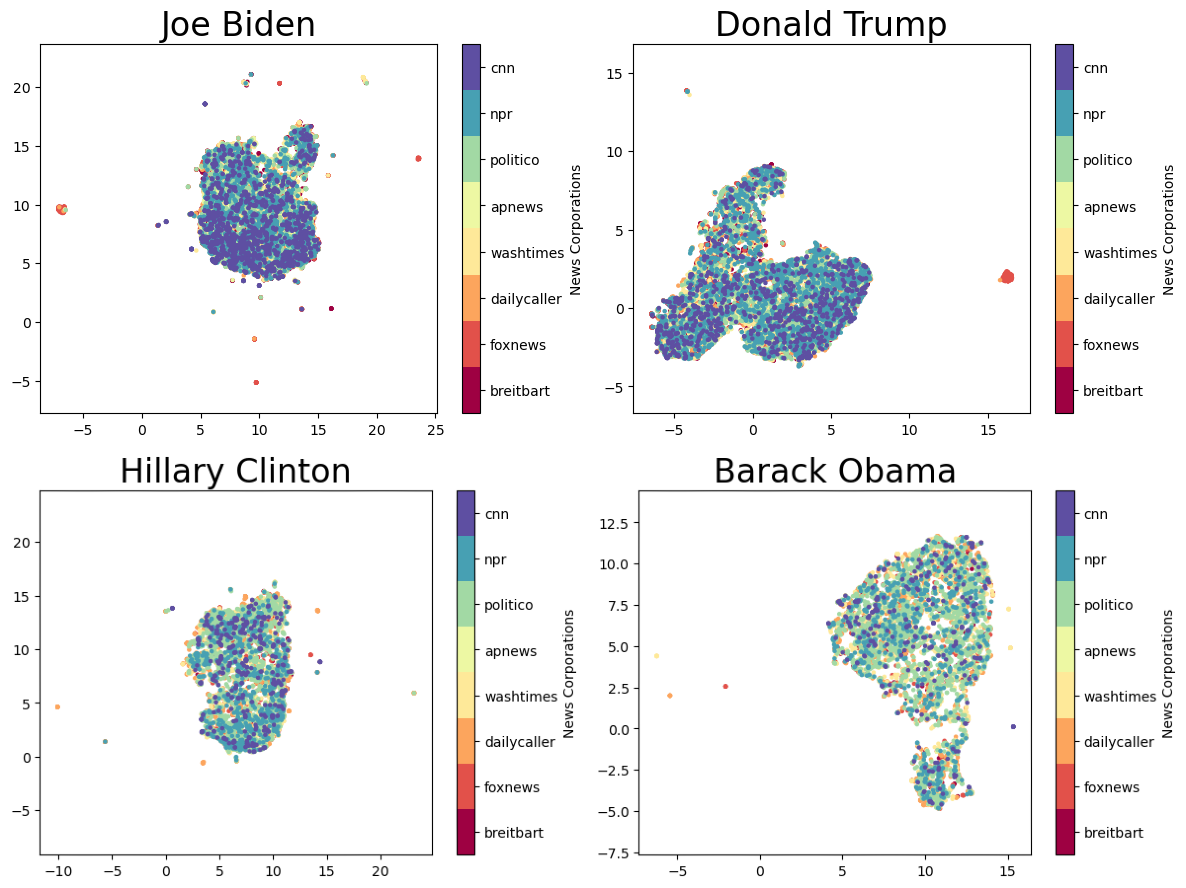
\includegraphics[width=.5\textwidth]{assets/emotion_cor.png}
    \caption{Emotion Logits with News Corporations as label \newline Remark: There is a small group of outliers to the left of Joe Biden's emotion logit plot and a group to the right of Donald Trump's emotion logit plot. The sources of the two groups are both Fox News, and the source images from each group are exactly the same. These are examples that news corporations may reuse some images for multiple time.}
    \label{fig:emo_cors}
    \vspace{10pt}
\end{figure}

\begin{figure}
    \centering
    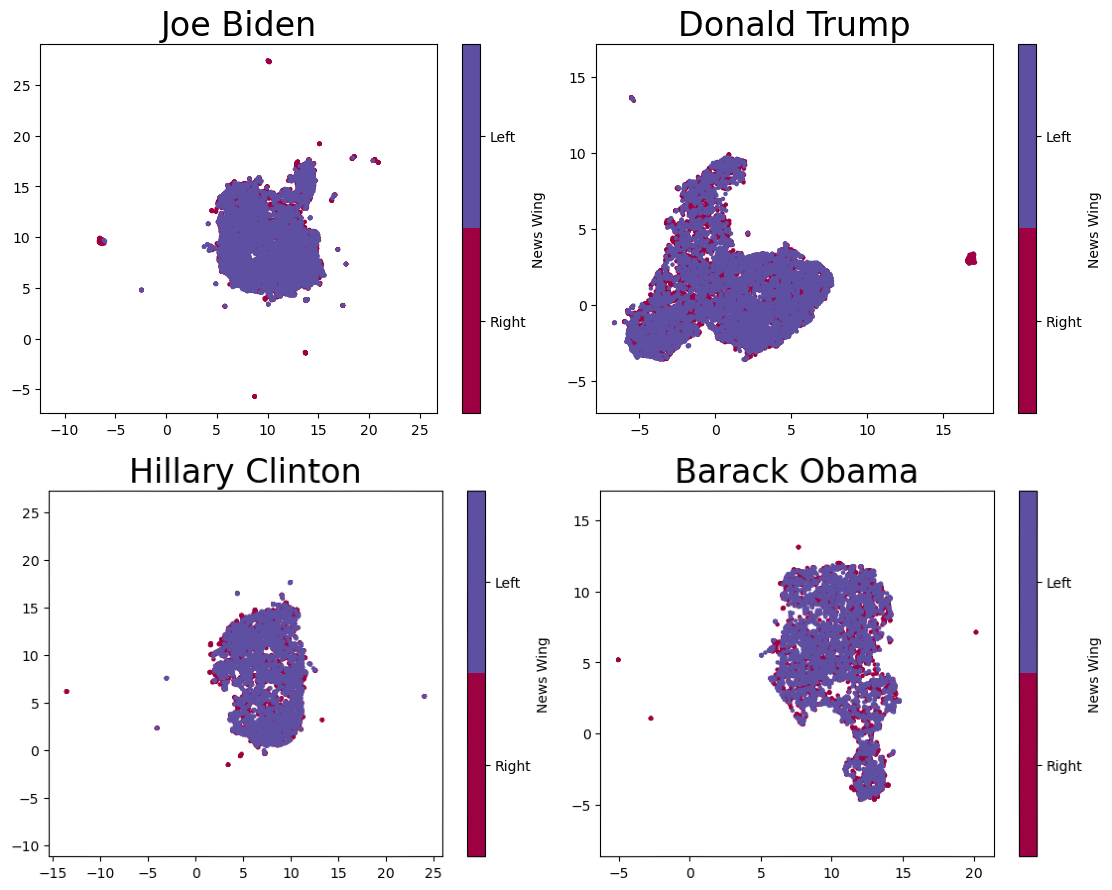
\includegraphics[width=.5\textwidth]{assets/emotion_bias.png}
    \caption{Emotion Logits with the Political Bias of News Corporations as label}
    \label{fig:emo_bias}
    \vspace{10pt}
\end{figure}


For visualization, we employ the UMAP technique, as done in previous sections, to reduce the dimensionality of emotion logits for each politician and label them by news corporation, as illustrated in Figure ~\ref{fig:emo_cors}. The color bar reflects the political spectrum of news media, ranging from progressive to conservative. The plots reveal that emotion logits from different corporations significantly overlap, indicating that it is challenging to distinguish between news sources based solely on emotion logits.

Additionally, we categorized the eight news corporations by their political biases as outlined in Table ~\ref{tab:source}. Specifically, CNN, NPR, Politico, and AP News represent left-leaning media, while the Washington Times, the Daily Caller, Fox News, and Breitbart are categorized as right-leaning. When re-plotting the emotion logits with political bias labels as shown in Figure ~\ref{fig:emo_bias}, the data still shows considerable overlap across different political biases, suggesting that emotion logits alone may not be sufficient to classify the political leanings of the media.

We also employed the PCA method for dimension reduction and analyzed the emotion probability vectors (obtained by applying the softmax function to the emotion logits). These plots, presented in the Appendix ~\ref{sec:vis_pca} and ~\ref{sec:prob}, consistently show overlapping emotion vectors across different news corporations and political biases. This overlap suggests a uniformity in the portrayal of emotions of each politician across diverse news corporation, despite differing political affiliations.


\subsection{Classification of Emotion Logits}\label{sec:classification}
While visualizing the dimension-reduced emotion logits offers intuitive insights, the two-dimensional vector representation may not fully capture the nuanced features of the original seven-dimensional emotion logits. To address this, we implemented a KNN classification model for each politician's emotion logits, labeling them by news corporation. We partitioned the data into training and validation sets in a 3:1 ratio, trained a KNN model with \(K=20\), and then evaluated the validation accuracy against a baseline. Additionally, we visualized the emotion logits of the validation set with predicted corporation labels and analyzed the confusion matrix. The results are detailed in Table ~\ref{tab:test_cor} and Figure ~\ref{fig:test_vis}.

\begin{table}[ht]
  \centering
  \renewcommand{\arraystretch}{1.2}
  \begin{tabular}{|l|l|r|}
    \hline
    \textbf{Politician} & \textbf{Baseline accuracy} & \textbf{Validation accuracy} \\ \hline
    Joe Biden & 0.1502 & 0.2589 \\ \hline
    Donald Trump & 0.1530 & 0.2444 \\ \hline
    Hillary Clinton & 0.2789 & 0.3765 \\ \hline
    Barack Obama & 0.2874 & 0.3328 \\ \hline
  \end{tabular}
  \caption{Baseline and Validation Accuracy for Predicting the Source Corporations from Emotion Logits}
  \label{tab:test_cor}
\end{table}

\begin{figure}
    \centering
    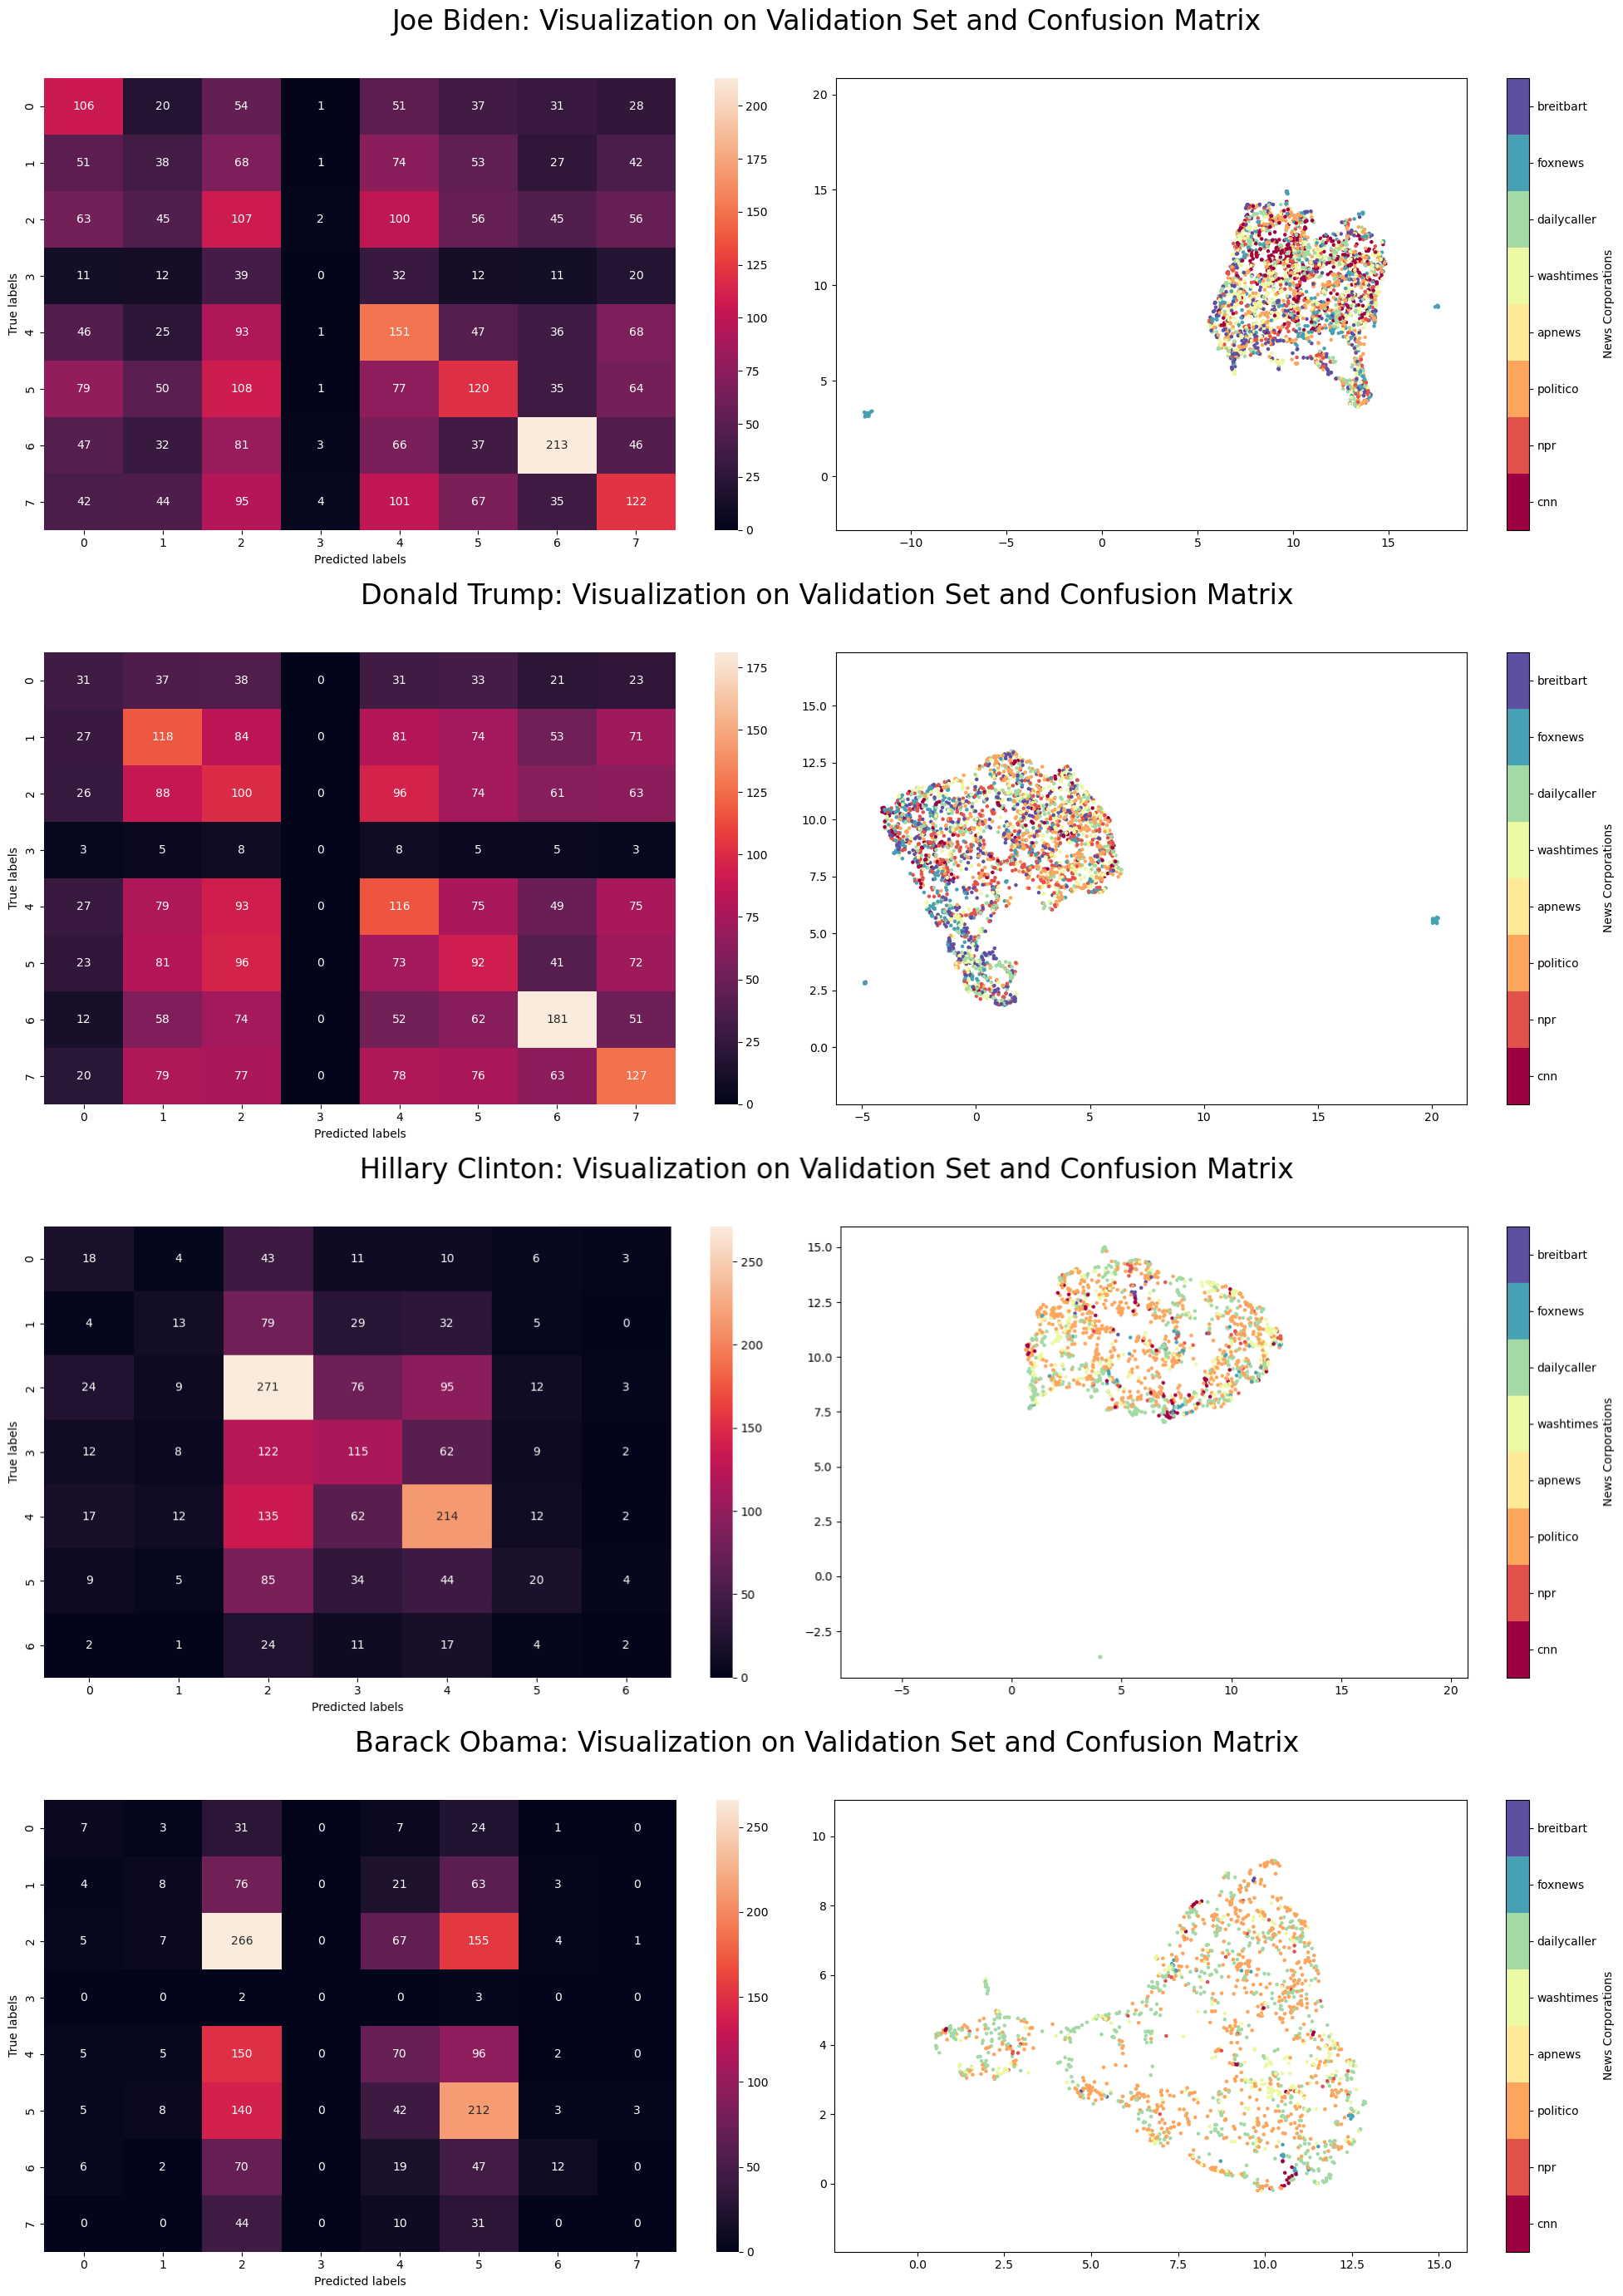
\includegraphics[width=.5\textwidth]{assets/test_cm_cor.png}
    \caption{Confusion Matrices and Visualization of Predicted Corporation of Validation Set \newline Remark: Due to only one emotion logit being available for Hillary Clinton labelled AP News, the confusion matrix for her is constrained to a 7x7 size. }
    \label{fig:test_vis}
    \vspace{10pt}
\end{figure}

The Baseline accuracy here is defined as naively choosing the category with most samples. According to Table ~\ref{tab:test_cor}, the validation accuracy for each politician remains relatively low, indicating the inaccuracy on predicting news corporations based on emotion logits using the KNN model. Besides, when examining the confusion matrices (Figure ~\ref{fig:test_vis}, left column), we found for each politicians, despite the dark rows and columns (which stands for there are inadequate data from the corresponding news resource), the brightness of each entries are similar, which means the high probability of wrongly prediction. Additionally, the visual plots of predicted news sources (Figure ~\ref{fig:test_vis}, right column) with the emotion logits in the validation set after reducing dimension with UMAP show no clear boundaries between clusters, suggesting significant overlap in the portrayal of emotion logits across different corporations.


It might be observed that the validation accuracies are somewhat higher than the baseline accuracies, as shown in Table ~\ref{tab:test_cor}, and that the diagonals of each confusion matrix are slightly more highlighted than the off-diagonal entries. One explanation for these observations, as discussed in Section ~\ref{sec:data}, is that some news corporations may reuse the same images (with same URL) across multiple articles. Although our analysis accounts for these duplicates, the underlying reasons for image reuse by news corporations may extend beyond a preference for certain expressions. Such reasons could include operational efficiencies, such as optimizing image storage, or consistency in coverage of specific events. An example of this is the outliers mentioned in the caption of Figure ~\ref{fig:emo_cors}. The KNN model's methodology, which involves voting among the 20 closest neighbors, may lead to an apparent increase in prediction accuracy. However, this could be misleading and might be indicative of overfitting.

Consequently, with the usage of KNN classification model, we still could not predict the source news corporations based on the emotion logits for each politician.

Besides news corporations individually, we are interested in determining if we can classify the emotion logits based on the political bias of the news corporations, divided into left and right groups. We divided the eight corporations accordingly, split the data into training and validation sets in a 3:1 ratio, and trained a KNN model with \(K=20\). The results, including validation accuracy, confusion matrices, and plots of the predicted political bias from the validation set, are presented in Table ~\ref{tab:test_bias} and Figure ~\ref{fig:test_vis_bias}.

\begin{table}[ht]
  \centering
  \renewcommand{\arraystretch}{1.2}
  \begin{tabular}{|l|l|r|}
    \hline
    \textbf{Politician} & \textbf{Baseline accuracy} & \textbf{Validation accuracy} \\ \hline
    Joe Biden & 0.6008 & 0.5939 \\ \hline
    Donald Trump & 0.6119 & 0.5983 \\ \hline
    Hillary Clinton & 0.5669 & 0.6319 \\ \hline
    Barack Obama & 0.5701 & 0.5655 \\ \hline
  \end{tabular}
  \caption{Baseline and Validation Accuracy for Predicting the Political Bias of Source Corporations from Emotion Logits}
  \label{tab:test_bias}
\end{table}

\begin{figure}
    \centering
    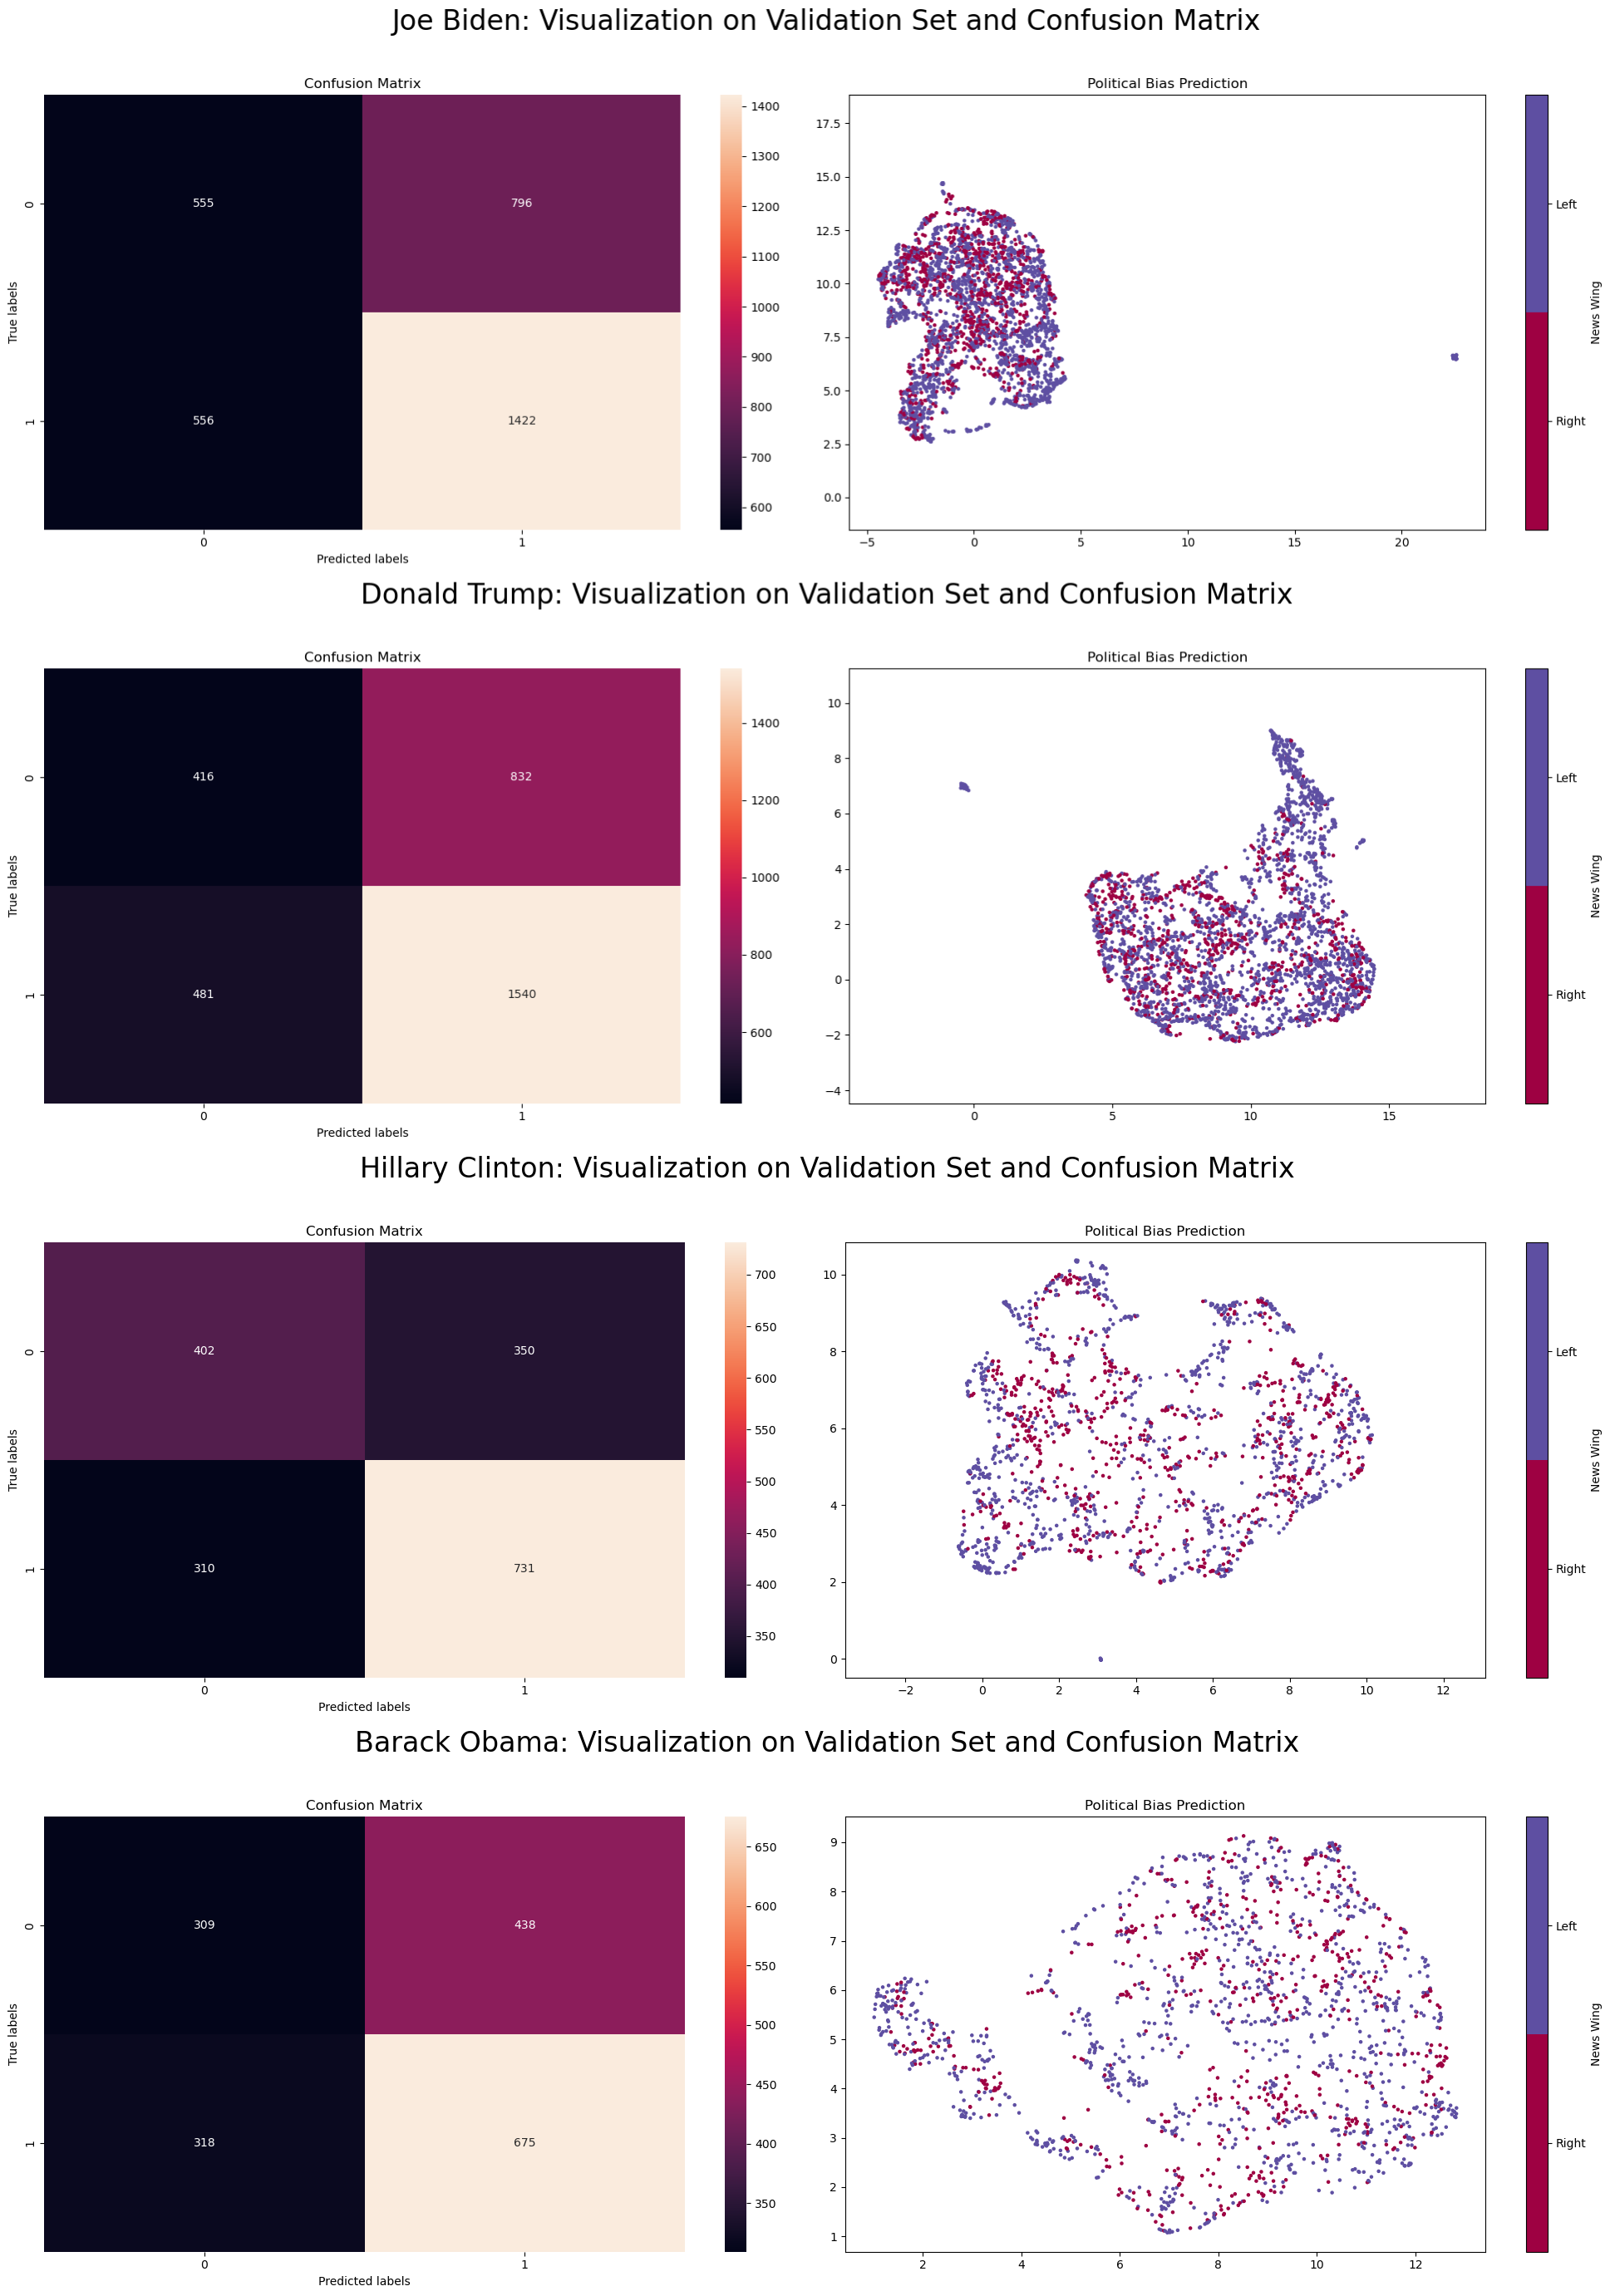
\includegraphics[width=.5\textwidth]{assets/test_cm_bias.png}
    \caption{Confusion Matrices and Visualization of Predicted Political Bias of Validation Set}
    \label{fig:test_vis_bias}
    \vspace{10pt}
\end{figure}


Notably, the validation accuracy of the KNN model for each politician is nearly equivalent to the baseline accuracy. The scatter plots reveal that the emotion logits of the two predicted groups, after dimension reduction via UMAP, are indistinguishably distributed, indicating that the groups are not effectively distinguishable by the model. This suggests a significant overlap in the portrayal of emotions, irrespective of the political bias of the news sources. Additionally, we include the results of the classification analysis for a wider range of politicians in Appendix ~\ref{sec:more}, which are consistent with the conclusions.

\vspace{-10pt}

\section{Discussion}\label{sec:discussion}

\subsection{Impact of Remaining Duplicates on Conclusions} \label{sec:duplicates}
In Section ~\ref{sec:clean}, we addressed the presence of various forms of duplicate data within our dataset—some duplicates were removed, while others remained due to limitations in identifying them. A particular challenge involves instances where different URLs point to the same news article within a corporation, potentially featuring resized images or differing textual content. Without access to the original articles, it is impractical to identify and remove these duplicates.

However, the research experiments and results we obtained told that the duplicates in the cleaned dataset would not affect the conclusion. The presence of duplicates might typically lead to overfitting in our models; however, our analyses indicate that even with potential overfitting, the models are unable to effectively distinguish between categories. This suggests that even an ideal model, devoid of any overfitting, would likely reach the same conclusion

For instance, suppose duplicated images with faces in our dataset produce closely aligned emotion logits. These logits, when subjected to dimension reduction via UMAP, would cluster together on the plot. Furthermore, given that KNN is a non-parametric voting mechanism, duplicated logits in the validation set are more likely to be predicted accurately, as they resemble those in the training set. Thus, any duplication tends to reinforce a pattern where high validation accuracy would indicate successful classification, suggesting overfitting. However, as detailed in Section ~\ref{sec:results}, the emotion logits across different news corporations and political biases do not exhibit distinct clustering, pointing to their non-distinguishability.

Therefore, even if we were to eliminate all remaining duplicates from the dataset, the overarching conclusion that emotion logits cannot reliably distinguish between the political biases or corporate sources of news images would remain unchanged. 



\subsection{Possible Reasons of the Results}
In this subsection, I will discuss potential underlying reasons why our results unfolded as they did.

\subsubsection{Lack of Deliberate Selection of Facial Expressions by News Corporations} 



One plausible explanation for our results is that news corporations may not consistently choose photos of politicians with specific facial expressions, particularly negative ones. While previous research has shown that media can influence viewers' perceptions of candidates during elections by selecting images that convey different emotional expressions \cite{imagebite}, it may not be a sustainable strategy for larger news organizations to deliberately use photos with negative expressions for politicians they do not support.

Most readers seek out news that they perceive as relatively neutral. If a news corporation were to overtly display political bias by consistently choosing unflattering photos of influential politicians, it might risk alienating its existing audience. Furthermore, large news organizations are typically driven to increase their revenue by expanding their reader base, which often involves focusing more on the content of their news articles and political commentaries rather than subtle cues like photo selection. This strategic choice could explain why the emotion logits of images from different news sources do not distinctly classify into separate groups based on the political bias or source of the news corporation.


\subsubsection{Limited Representation of Political Bias Across News Corporations}

As indicated in Table ~\ref{tab:source}, our dataset comprises samples from eight news corporations, yet it lacks representation from several major mainstream outlets, such as The New York Times, The Wall Street Journal, The Washington Post, and the New York Post. Consequently, relying solely on these eight media sources may not adequately capture the full spectrum of political bias present in the U.S. media landscape.

Moreover, the distribution of samples within our dataset is uneven across the political spectrum. The four right-leaning media sources contribute approximately 100,000 samples each, evenly distributed. In contrast, the sample distribution among the left-leaning sources is disproportionately skewed; Politico alone contributes 312,000 samples, significantly outnumbering the combined total from the other three left-leaning outlets. This imbalance was particularly evident in our experimental results: for politicians other than Joe Biden and Donald Trump, the majority of samples attributed to left-leaning media originated from Politico. This skew is observable in the darker columns of the confusion matrix presented in Figure ~\ref{fig:test_vis}. Such a disparity not only challenges the balance of our dataset but may also lead to underfitting in our models, as the overwhelming prevalence of samples from a single source may not provide a sufficiently diverse foundation for generalizing across other news corporations.




\subsubsection{Inadequate Representation of Facial Expressions by Emotion Logits}

In our study, facial expressions are represented as seven-dimensional emotion logits, encapsulating the combination of six basic emotions and a neutral expression \cite{compoundemotion}. However, actual facial expressions are controlled by a complex system involving 20-30 muscles on each side of the face \cite{muscle}, suggesting that a 7-dimensional vector may not sufficiently capture the full range of human facial expressions.

Additionally, the perception of emotions from facial expressions can be subjective. Different individuals may interpret the same facial expression in varied ways. Coupled with the inherent error rate of the RMN model used to interpret these expressions, the emotion logits may not be considered an absolute measure of facial expressions. This subjective nature and potential inaccuracies in emotion recognition technology might contribute to the inability of our models to distinctly classify images based on the emotion logits derived from facial expressions.



\subsubsection{Same expression may have different meaning}

As previously discussed, the interpretation of facial expressions can vary significantly across different news corporations. For instance, our analysis of the emotion logits dataset reveals that the dominant facial expression ((i.e. the label with maximum of average emotion logits) for Donald Trump across all eight news corporations is categorized as "angry."  This uniformity in expression categorization does not necessarily imply a consensus on its meaning or implication.

For example, if we hypothesize that these news corporations are selectively using images where Trump appears angry, it is plausible to interpret their motivations differently based on their political orientation. Progressive media might select such images to portray Trump as irritable and agitated, aligning with a narrative that criticizes his temperament and suitability for leadership. Conversely, conservative media could be using the same expression to emphasize his passion and assertiveness, traits that are often celebrated by his supporters as signs of strength and decisiveness.

This divergence in interpretation highlights a complex layer of media bias where the same visual information can be framed in completely different contexts. Each news corporation may choose similar expressions but for entirely different reasons, aiming to reinforce specific narratives that resonate with their respective audiences. 



\subsubsection{The Impact of Timing on Photo Selection}

Our dataset does not include the publication dates of the news articles from which the images were sourced. This omission limits our ability to analyze how the selection of facial expressions for certain politicians might change over time due to evolving political contexts. A pertinent example is Mike Pence, who served as Vice President under Donald Trump from 2016 to 2020. During most of his term, Pence was seen as a loyal ally of Trump, but his relationship with Trump soured post the 2020 election. If a news corporation’s portrayal of Pence shifted from positive to negative in response to these events, the overall effect could neutralize the perceived emotion in images of him over time. This dynamic is especially relevant for the Trumpophile outlets; they might initially select images that cast Pence in a favorable light, only to choose more critical representations later, effectively averaging the portrayed emotions to appear neutral. This phenomenon underscores the potential influence of temporal context on the media's selection of images, which could significantly affect the interpretation of political figures' facial expressions.




\subsection{Future Work}


To build on the findings of our current research, our first step in future work will involve creating a more comprehensive dataset that includes a wider range of news corporations. This dataset will not only encompass a larger sample size for each included news outlet but will also aim to incorporate the publication dates of the articles from which the images are sourced. The addition of timestamps will allow us to examine how media portrayal of the facial expression of politicians may shift over time, potentially in response to political events or changes in public perception. This temporal dimension could provide deeper insights into the strategies news corporations employ in their visual representation of political figures.

In our subsequent studies, we plan to move beyond the use of emotion logits for facial expression analysis. Instead, we will explore the application of more sophisticated facial feature recognition models that can process face crops and generate higher-dimensional vectors. These vectors will capture a broader array of facial features, potentially offering a more nuanced understanding of the expressions depicted in media images. By employing these advanced vectors, we aim to refine our analysis and improve the accuracy of our interpretations of media bias and facial expression portrayal.

While our current research focuses primarily on politicians, there is significant potential to expand this approach to other public celebrity, such as prominent business leaders. For example, analyzing media images of figures like Elon Musk could reveal interesting patterns in how business personalities are visually represented in the medias with different political bias, which may differ significantly from political figures. This expansion would not only diversify our research but also enhance our understanding of media bias and representation across different sectors.

To support these enhancements, we are considering the implementation of Amazon Rekognition. This AWS service offers robust pretrained models that are highly effective in recognizing the names of celebrities and analyzing facial features\cite{reko}. By leveraging Amazon Rekognition, we can benefit from its advanced machine learning capabilities to accurately identify public figures and their facial expressions in media images. This technology will provide a more reliable and scalable method for conducting our analyses, potentially increasing both the efficiency and the breadth of our research into media representations.


\vspace{-10pt}
\section{Conclusion}\label{sec:conclusion}

Throughout our study, we developed a name recognition model using image data from the pages of politicians in Wikimedia and Wikipedia, which we then applied to our dataset to retrieve and extract face crops of influential politicians. Subsequently, we generate emotion logits corresponding to each politicians and each news corporation. With analyzing the emotion logits, our results indicate that there is no clear relationship between the facial expressions of specific politicians in media images and news corporations or their political bias.

While our findings suggest that news corporations might not use facial expressions strategically to align with their political biases, this does not diminish the complexity and potential subtleties in how news media use images to influence public perception. This research paves the way for more detailed examinations of how visual media influences political and public attitudes, highlighting the necessity for advanced techniques and tools to explore the relationship between media images and editorial inclination.



%%
%% The acknowledgments section is defined using the "acks" environment
%% (and NOT an unnumbered section). This ensures the proper
%% identification of the section in the article metadata, and the
%% consistent spelling of the heading.
\begin{acks}
We extend our thanks to Prof. Jame Turk, for providing with the interesting and inspiring research topic with dataset; my advisor Prof. Aaron Schein, for giving instructions and suggestions during the research period; and Dr. Patricia Chiril, for discussing the different approaches of the topic and cross verify the results.
\end{acks}


\section*{REPRODUCIBILITY}
All codes we used for this research is available at \href{https://github.com/Chenfeng-Li/Politician-Image-Project}{\underline{https://github.com/}} \href{https://github.com/Chenfeng-Li/Politician-Image-Project}{\underline{Chenfeng-Li/Politician-Image-Project}}. Please follow the instruction in README.md file for reproducing.


%%
%% The next two lines define the bibliography style to be used, and
%% the bibliography file.
\bibliographystyle{ACM-Reference-Format}
\bibliography{biblio}


%%
%% If your work has an appendix, this is the place to put it.
\section*{Appendix}
\appendix

\section{Visualization using PCA}\label{sec:vis_pca}
In this appendix section, we explore an alternative method for dimension reduction by implementing PCA, in contrast to the UMAP technique discussed in Section ~\ref{sec:vis}. We continue to use the labels of news corporations and political bias for the plots. The resultant PCA visualizations are displayed in Figure ~\ref{fig:emo_cors_pca} and Figure ~\ref{fig:emo_bias_pca}. These plots demonstrate that the emotion logits for different groups are nearly indistinguishable, with a high degree of overlap and similar distributions observed across categories. Consequently, these findings corroborate our earlier results, indicating that it is challenging to discern the news corporation or political bias based solely on emotion logits.

\begin{figure}
\centering
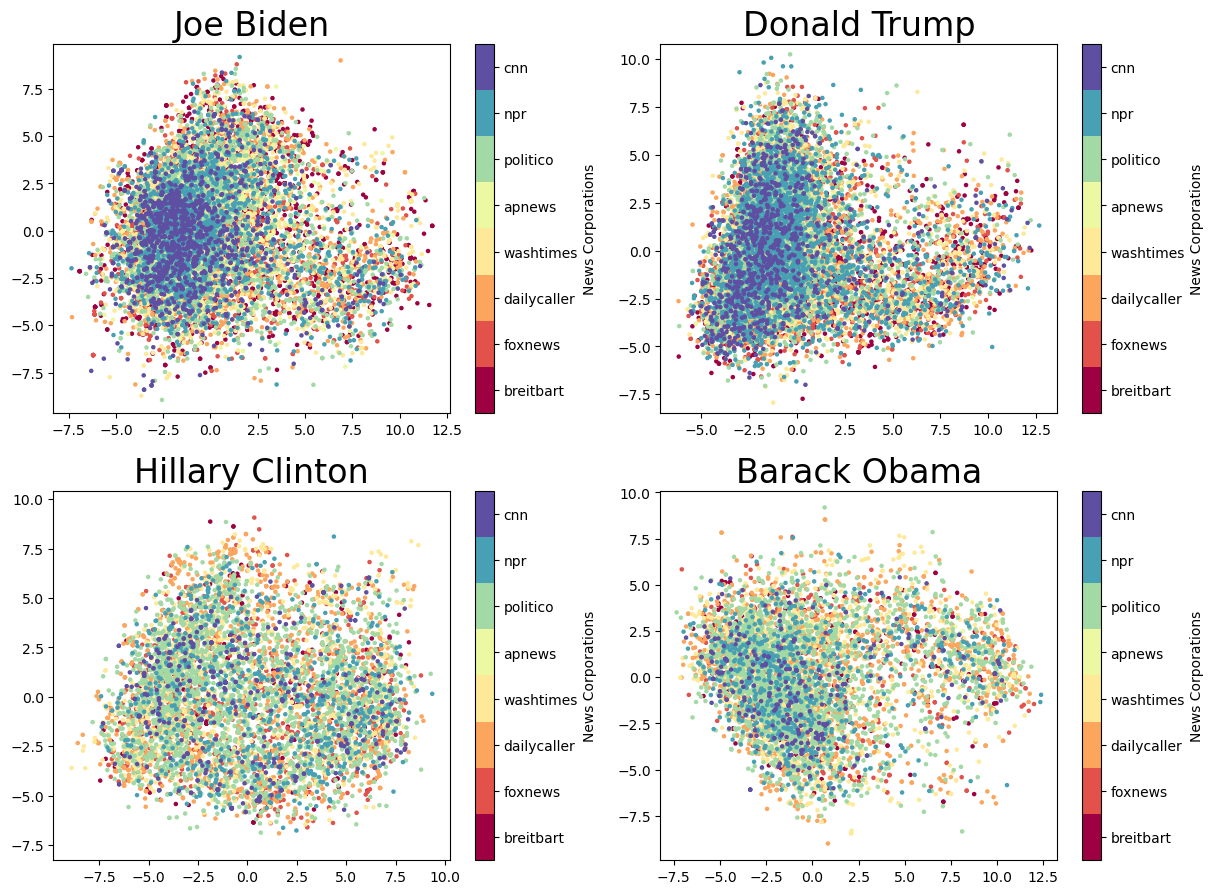
\includegraphics[width=.5\textwidth]{assets/emotion_cor_pca.png}
\caption{Visualization of Emotion Logits with News Corporations as labels, using PCA for dimension reduction.}
\label{fig:emo_cors_pca}
\vspace{10pt}
\end{figure}

\begin{figure}
\centering
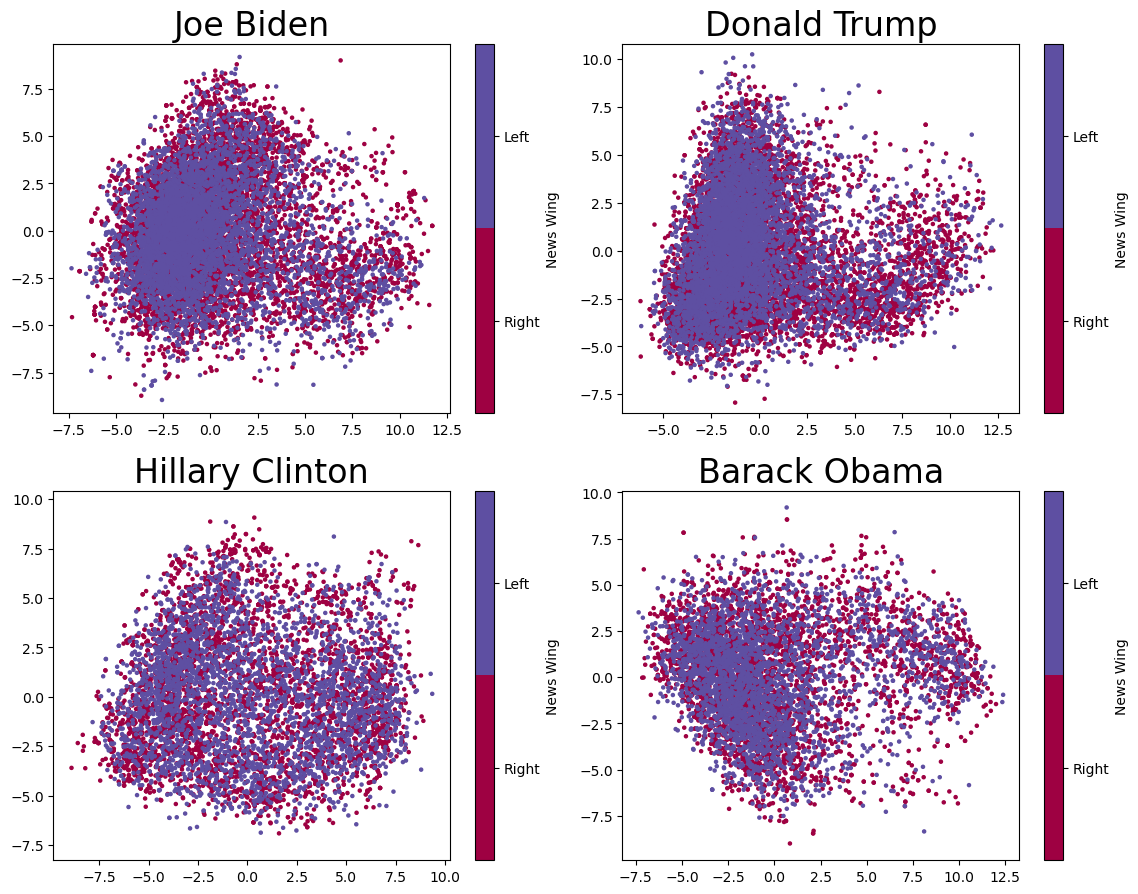
\includegraphics[width=.5\textwidth]{assets/emotion_bias_pca.png}
\caption{Visualization of Emotion Logits with the Political Bias of News Corporations as labels, using PCA for dimension reduction.}
\label{fig:emo_bias_pca}
\vspace{10pt}
\end{figure}



\section{Visualiztion of emotion probabilities}\label{sec:prob}
In the main body of this paper, we primarily analyzed emotion logits. In this section, we briefly show the results of converting these logits into emotion probabilities, defined through the softmax function:

\[
\text{Emotion Probability} = \text{softmax(Emotion Logit)}
\]

\[ 
\text{softmax}(\boldsymbol{x}) = (\frac{exp(x_1)}{\sum_{j} exp(x_j)}
,\dots,(\frac{exp(x_n)}{\sum_{j} exp(x_j)})
\]

As in previous analyses, we employ UMAP for dimension reduction to visualize the emotion probabilities, labeling them according to their corresponding news corporations or political biases. The resulting visualizations are displayed in Figure ~\ref{fig:emo_cors_prob} and Figure ~\ref{fig:emo_bias_prob}. Given that probability vectors are constrained (the sum of the entries must equal one), the shapes of the plots post-dimension reduction appear irregular. From these plots, it is evident that the probability vectors within each category significantly overlap. 


\begin{figure}
\centering
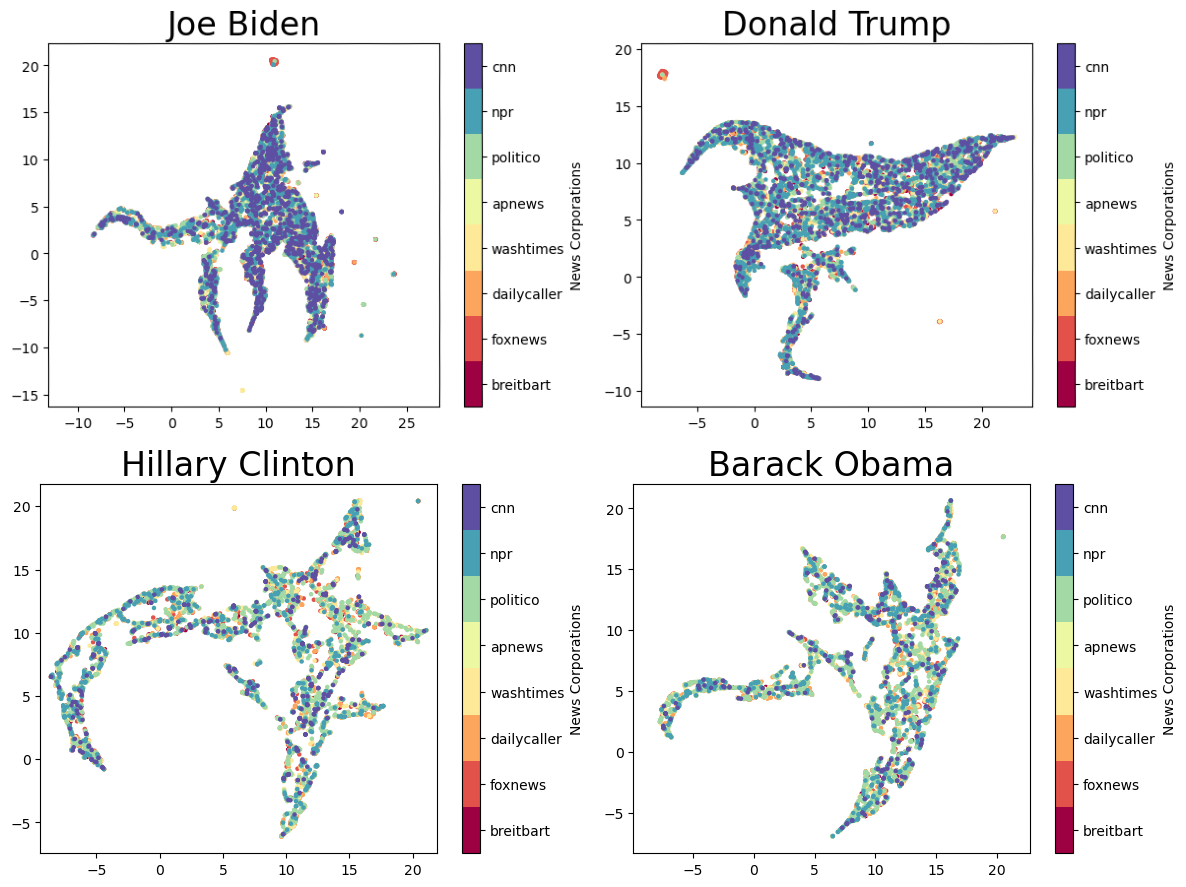
\includegraphics[width=.5\textwidth]{assets/emotion_cors_prob.png}
\caption{Visualization of Emotion Probabilities with News Corporations as labels.}
\label{fig:emo_cors_prob}
\vspace{10pt}
\end{figure}

\begin{figure}
\centering
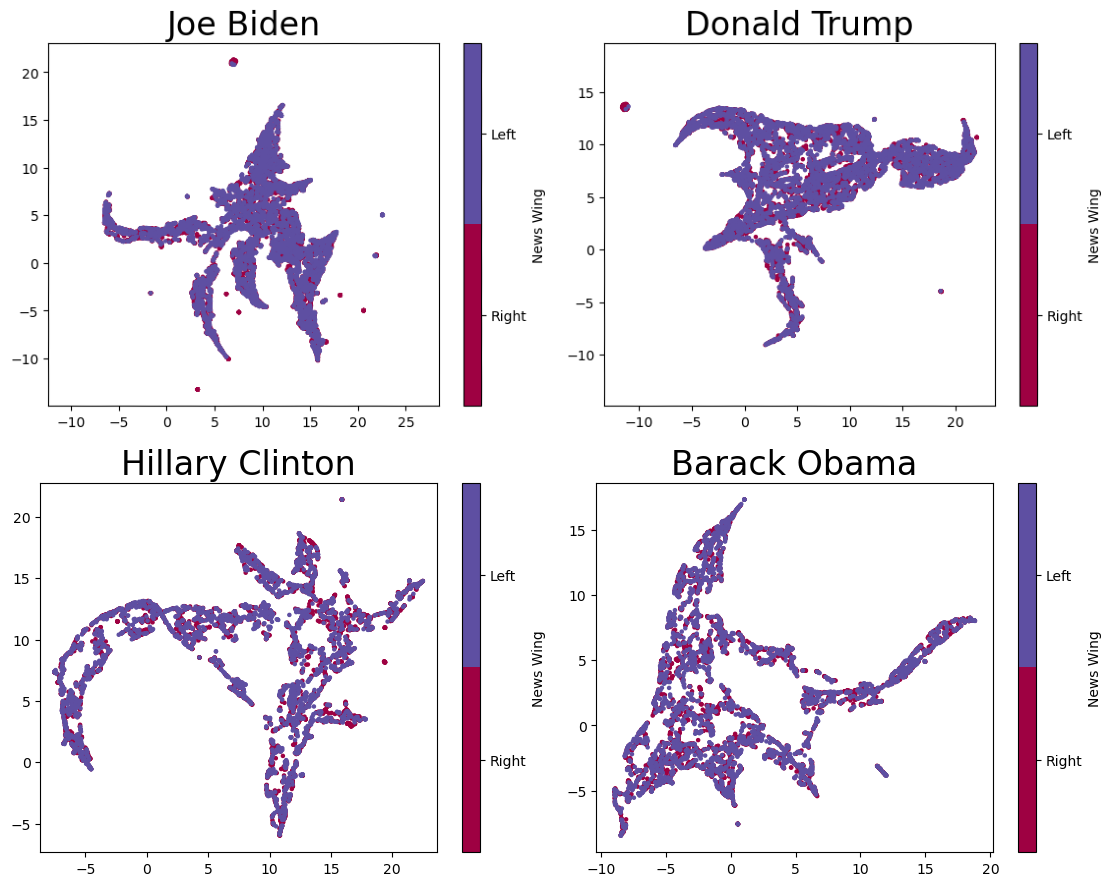
\includegraphics[width=.5\textwidth]{assets/emotion_bias_prob.png}
\caption{Visualization of Emotion Probabilities with with the Political Bias of News Corporations as labels.}
\label{fig:emo_bias_prob}
\vspace{10pt}
\end{figure}

Thus, we conclude that even when transformed into probabilities, the data still fails to distinguish between news corporations or political biases effectively.

\section{Classification Analysis for Additional Politicians}\label{sec:more}

In Section ~\ref{sec:classification}, we discussed the classification results for Joe Biden, Donald Trump, Hillary Clinton, and Barack Obama. In this section, we extend the analysis to include more influential politicians, implementing classification analyses on their emotion logits with news corporations or political biases as labels. The results are presented in Tables ~\ref{tab:test_cor_more} and ~\ref{tab:test_bias_more}, where we detail the total sample size of emotion logits for each politician across all eight news corporations, and the sample sizes from left-leaning and right-leaning news corporations, respectively. Notably, as per the constraints mentioned in Section ~\ref{sec:facecrops}, we collected a maximum of 2,000 emotion logits per politician for each news corporation. The results affirm that our initial conclusions remain unchanged.


\begin{table}[H]
  \centering
  \renewcommand{\arraystretch}{1.2}
  \begin{tabular}{|l|l|l|r|}
    \hline
    \textbf{Politician} & \textbf{\makecell{Total \\Sample Size}} & \textbf{\makecell{Baseline \\ accuracy}} & \textbf{\makecell{Validation\\ accuracy}} \\ \hline
    Joe Biden & 13316 &  0.1502 & 0.2589 \\ \hline
    Donald Trump & 13034 &  0.1530 & 0.2444 \\ \hline
    Hillary Clinton & 7171 &  0.2789 & 0.3765 \\ \hline
    Barack Obama & 6959 &  0.2874 & 0.3328 \\ \hline
    Kamala Harris & 4596 & 0.3068 & 0.5030 \\ \hline
    Kevin McCarthy & 3562 & 0.3565 & 0.6083 \\ \hline
    Mike Pence & 5853 & 0.3417 & 0.5689 \\ \hline
    Nancy Pelosi & 7440 & 0.2688 & 0.3935 \\ \hline
    Antony Blinken & 620 & 0.3210 & 0.3806 \\ \hline
    Mitch McConnell & 4741 & 0.3450 & 0.4391 \\ \hline
    Ted Cruz & 3938 & 0.3999  & 0.4569 \\ \hline
    
  \end{tabular}
  \caption{Classification Analysis of News Corporation}
  \label{tab:test_cor_more}
\end{table}

\begin{table}[H]
  \centering
  \renewcommand{\arraystretch}{1.2}
  \begin{tabular}{|l|l|l|r|}
    \hline
    \textbf{Politician} & \textbf{\makecell{Sample Sizes of Left\\and Right Medias}} & \textbf{\makecell{Baseline \\ accuracy}} & \textbf{\makecell{Validation\\ accuracy}} \\ \hline
    Joe Biden & 5316, 8000 & 0.6008 & 0.5939 \\ \hline
    Donald Trump & 5074, 8000 & 0.6119 & 0.5983 \\ \hline
    Hillary Clinton & 3106, 4065 & 0.5669 & 0.6319 \\ \hline
    Barack Obama & 2992, 3967 &  0.5701 & 0.5655 \\ \hline
    Kamala Harris & 1357, 3239 & 0.7047 & 0.6963 \\ \hline
    Kevin McCarthy & 1105, 2457 & 0.6897 & 0.7138 \\ \hline
    Mike Pence & 1991, 3862 & 0.6598 & 0.6790 \\ \hline
    Nancy Pelosi & 2200, 5240 & 0.7043 & 0.7091 \\ \hline
    Antony Blinken & 288, 332 & 0.5355 & 0.6903 \\ \hline
    Mitch McConnell & 1849, 2322 & 0.5567 & 0.6012 \\ \hline
    Ted Cruz & 2128, 1810 &0.5404 & 0.6173 \\ \hline
    
  \end{tabular}
  \caption{Classification Analysis of Political Bias}
  \label{tab:test_bias_more}
\end{table}

\end{document}
